\documentclass[a4paper,12pt]{book}
\usepackage[utf8]{inputenc}

\usepackage{amsmath, amssymb, enumitem, bm, xcolor, braket, dsfont, graphicx}
\usepackage[colorlinks, linkcolor = red, citecolor = black, filecolor = black, urlcolor = blue]{hyperref} 

% Quotes
\usepackage{epigraph}
\setlength\epigraphwidth{12cm}
\setlength\epigraphrule{0pt}

% \usepackage{mathptmx}
\usepackage{setspace}
%\singlespacing
\onehalfspacing

\renewcommand{\t}[1]{\text{#1}}
\renewcommand{\d}{{\rm d}}
\renewcommand{\b}[1]{\boldsymbol{#1}}
\newcommand{\B}[1]{\mathbf{#1}}
\newcommand{\D}[1]{{#1}^\dagger}
\newcommand{\fD}[1]{{#1}^{ \phantom{\dagger}}}
\renewcommand{\P}[1]{{#1}^\prime}
\newcommand{\fP}[1]{{#1}^{\phantom{\prime}}}
\newcommand{\im}{{\rm i}}
\newcommand{\halb}{\frac{1}{2}}

% transpose
\usepackage{relsize}
\newcommand{\tp}[1]{{#1}^{\mathrm t}}
% \!\: = 1mu distance; \!\; = 2mu (\, = 3mu)
\newcommand{\itp}[1]{{#1}^{\!\:\scalebox{0.55}[1.0]{\( - \)}1 \mathrm t}}

% comments:
\definecolor{dblue}{RGB}{31,119,180}
\newcommand{\REM}[1]{\textcolor{blue}{{\bf #1}}}
\newcommand{\CITE}[1]{\textcolor{blue}{{\bf [#1]}}}
% \newcommand{\FK}[1]{\textcolor{blue}{{\bf #1 }}}

\usepackage{blindtext}

% theorems
\usepackage{amsthm}
\newtheorem*{theorem}{Theorem}
\newtheorem*{thm}{Theorem}

% https://en.wikibooks.org/wiki/LaTeX/Title_Creation
\title{
    Thermal Conductivities of Strongly Anharmonic Compounds from First Principles
}
\author{
    Florian Knoop
    \\ \and
    First Supervisor: Prof. Dr. Claudia Draxl
    \and
    Second Supervisor: Prof. Dr. Matthias Scheffler
    \\ \and
    Fritz-Haber-Institut der Max-Planck-Gesellschaft, Berlin
}
\date{2020}

\begin{document}
\maketitle
\tableofcontents

\chapter{Introduction}
\epigraph{\singlespacing \it ``Die Zeit des unbedenklichen Wirtschaftens mit den Energiequellen und Stofflagern, die uns die Natur zur Verfügung gestellt hat, wird wahrscheinlich schon für unsere Kinder nur noch die Bedeutung einer vergangenen Wirtschaftsepoche haben.''}{W. Schottky, 1929}
% [ ] Why thermal conductivity?
% [ ] Why novel thermal insulators?
% [ ] Why computational materials science?
One of the major challenges humankind faces in the 21th century is the responsible and sustainable handling of the earth's natural resources~\cite{Schottky1929}.  Yet, most energy today is lost as waste heat during the transformation of raw energy sources to usable power. To date, there is no fuel based heat engine that exceeds an efficiency of 50\,\% and often it is even worse~\cite{eia}. 
Since gas- and aircraft-turbines are essentially Carnot engines, their efficiency and core power are directly related to the combustion temperature~\cite{Clarke2012,Perepezko2009}. This has been utilized during the past 30 years by developing 
ceramics with high thermal resistivity that are nowadays applied as \emph{thermal barrier coatings} on turbine airfoils in heat engines~\cite{Clarke2003}. A thermal barrier coating serves as a thin, extremely heat insulating layer and thus allows to operate a turbine at higher temperatures, thereby increasing its efficiency.

A complementary strategy is to recycle waste heat where it occurs. One way to do so is to use the
\emph{thermoelectric effect} to  generate electric power from temperature gradients~\cite{Snyder2008}. The main obstacle preventing mass operation though is the limited conversion rate (figure of merit) $zT$ of even the most advanced thermoelectric materials known to date. To make matters worse, these materials often contain heavy metals and are toxic, and their manufacturing process is difficult and expensive~\cite{Nolas2001}. Recent advancements in the field, such as the discovery of a high thermoelectric figure of merit in the lead-free material Tin Selenide~\cite{Zhao2014}, offer hope that novel materials with significant figure of merit can be found that are non-toxic, easy and cheap to produce, and consist of abundant elements.

A key physical property of both thermal barrier coatings (TBCs) and thermoelectrics is their thermal conductivity $\kappa$. In the case of thermoelectrics, the figure of merit is inversely proportional to $\kappa$~\cite{Nolas2001}:
\begin{align}
	zT = \frac{S^2 \sigma_{\rm el}}{\kappa} T~,
	\label{eq:zT}
\end{align} 
where $T$ dentoes the temperature, $S$ the Seebeck coefficient, and $\sigma_{\rm el}$ is the electrical conductivity.
A prerequisite to finding better thermoelectrics or TBCs therefore is to find materials which are thermally insulating. These are typically non-metals, since the free electrons in metals are good heat carriers, and most of the known thermoelectrics are thermally insulating inorganic semiconductors~\cite[p.\,15]{Nolas2001}.

% [ ] say sth. about microstructuring?

Despite the technological needs, systematic knowledge of thermal conductivities in inorganic compounds is scarce. A renowned database like Springer Materials only lists thermal conductivities for about 200~of these compounds~\cite{SpringerMaterials}, which is partially due to the fact that accurate measurements of thermal conductivity are tricky to perform[\REM{citation!}]. As a consequence, thermal conductivity is not systematically understood beyond semi-empirical and phenomenological trends in a very limited number of simple material classes~\cite{Morelli}.
\\ \\
The aim of this work is to open a new pathway for overcoming the problem of limited data by devising a route to systematically scan material space for thermal insulators and calculate their thermal conductivities from first principles. This route is twofold: After reviewing the relevant theoretical tools necessary to simulate heat transport in thermal insulators, we describe how to assess a key physical property shared by most thermal insulators,~.i.\,e.,~\emph{anharmonicity}, without the need for explicit model building beyond the harmonic approximation.

\chapter{Theory and Methods}

\section{The Many Body Problem}
\epigraph{\singlespacing \it ``The underlying physical laws necessary
for the mathematical theory of a large part of physics and the whole of chemistry
are thus completely known, and the difficulty is only that the exact application
of these laws leads to equations much too complicated to be soluble. It therefore becomes desirable that approximate practical methods of applying quantum
mechanics should be developed, which can lead to an explanation of the main
features of complex atomic systems without too much computation.''}{P.A.M. Dirac, 1929}

In this chapter, we summarize the theoretical background of {\it ab initio} simulations.

\subsection{The Many Body Hamiltonian}

The full (non-relativistic) many body Hamiltonian in the absence of external electromagnetic fields for an otherwise arbitrary system reads
\begin{align}
    \hat{\mathrm{H}}
        = \hat{\mathrm{T}}^{\mathrm{e}}
        + \hat{\mathrm{V}}^{\mathrm{e}-\mathrm{e}}
        + \hat{\mathrm{V}}^{\mathrm{e}-\mathrm{Nuc}}
        + \hat{\mathrm{V}}^{\mathrm{Nuc}-\mathrm{Nuc}}
        + \hat{\mathrm{T}}^{\mathrm{Nuc}}~,
    \label{eq:Hamiltonian}
\end{align}
where
\begin{align}
    \hat T^{\rm e} 
        =\sum_{i} \frac{\hat{\mathbf{p}}_{i}^{2}}{2 m_{\rm e}}
    \label{eq:Te}
\end{align}
is the kinetic energy operator for electrons of mass $m_{\rm e}$ with momentum operators $\hat{\bf p}_i$, and 
\begin{align}
    \hat V^{\rm e-e}
        = \sum_{i < j} \frac{e^{2}}{\left|\hat{\b r}_{i}-\hat{\bf r}_{j}\right|}~,
    \label{eq:Ve}
\end{align}
is the Coulombic electron-electron repulsion operator with the electronic position operators $\hat{\bf r}_i$ and the elementary charge $e$. 
The Coulomb attraction between the negatively charged electrons and the positively charged nuclei reads
\begin{align}
    \hat V^{\rm e-Nuc}
        = \sum_{i, J} -\frac{Z_J e^{2}}{\left|\hat{\b r}_{i}-\hat{\bf R}_{J}\right|}~,
    \label{eq:Venuc}
\end{align}
where $Z_J$ denotes the charge number of nucleus $J$, and $\hat{\bf R}_J$ is the nuclear position operator. 
Accordingly, we define the nuclear-nuclear repulsion as
\begin{align}
    \hat V^{\rm Nuc-Nuc}
        = \sum_{I < J} \frac{Z_{I} Z_{J} e^{2}}{\left|\hat{\b R}_{I}-\hat{\bf R}_{J}\right|}~,
    \label{eq:Vnuc}
\end{align}
and the kinetic energy operator for nuclei with momentum operators $\hat{\bf P}_I$ and masses $M_I$ reads
\begin{align}
    \hat T^{\rm Nuc} 
        =\sum_{I} \frac{\hat{\mathbf{P}}_{I}^{2}}{2 M_{I}}~.
    \label{eq:Tnuc}
\end{align}

\subsection{The Born Oppenheimer Approximation}
We go over to a unitless Hamiltonian by scaling Eq.\,\eqref{eq:Hamiltonian} with the Hartree energy $E_{\rm h} = me^4 / \hbar^2 \approx 27.2\,{\rm eV}$ and expressing distances in terms of the Bohr radius $a_0 = \hbar^2 / m e^2$,~i.\,e.,~${\bf r} = a_0 \tilde{\bf r}$, where $\hbar$ denotes the Planck constant~\CITE{Czycholl}. Dropping the operator hats in the following and using $\hat{\bf p}=-\im \hbar \partial / \partial {\bf r}$ instead, we have
\begin{align}
\begin{split}
    \tilde H 
        \equiv& ~H / E_{\rm h} \\
        =& 
        - \frac{1}{2} \sum_i \frac{\partial^2}{\partial \tilde{\bf r}_i^2}
        + \sum_{i < j} \frac{1}{\left|\tilde{\b r}_{i}-\tilde{\bf r}_{j}\right|}
        - \sum_{i, J} -\frac{Z_J}{\left|\tilde{\b r}_{i}-\tilde{\bf R}_{J}\right|}
        + \sum_{I < J} \frac{Z_{I} Z_{J}}{
            \left|\tilde{\b R}_{I}-\tilde{\bf R}_{J}\right|} 
        \\
        &- \frac{1}{2} \sum_I \frac{m_{\rm e}}{M_I} \frac{\partial^2}{\partial \tilde{\bf R}_I^2}~,
    \label{eq:Hscaled}
\end{split}
\end{align}
which only depends on the charge numbers $\{Z_I\}$ and the mass ratios $\{ m_{\rm e} / M_I \}$. The relative order of magnitude of the nuclear kinetic energy is $m_{\rm e} / M_I \approx 10^{-4} - 10^{-5}$. This means that the nuclear kinetic energy can be treated as a perturbation of the remaining electronic and electron-nuclear contributions:
\begin{align}
    H   &= H^0 + T^{\rm Nuc}~, \text{ where} 
    \label{eq:H=H0+T}
    \\
    H^0 &=
        {\mathrm{T}}^{\mathrm{e}}
        + {\mathrm{V}}^{\mathrm{e}-\mathrm{e}}
        + {\mathrm{V}}^{\mathrm{e}-\mathrm{Nuc}}
        + {\mathrm{V}}^{\mathrm{Nuc}-\mathrm{Nuc}}~.
    \label{eq:H0}
\end{align}
The full (time-independent) many-body Schroedinger equation reads
\begin{align}
    H \psi ({\bf r}, {\bf R}) = E \psi ({\bf r}, {\bf R})~,
    \label{eq:Schroedinger1}
\end{align}
with ground-state eigenvalues and many-body wave functions $E$ and \mbox{$\psi ({\bf r}, {\bf R})$},
where \mbox{${\bf r} = ({\bf r}_, \ldots, {\bf r}_{N_{\rm e}})$} denotes all electronic coordinates, and ${\bf R} = ({\bf R}_1, \ldots, {\bf R}_{N_{\rm Nuc}})$ all nuclear coordinates, respectively. According to Eq.\,\eqref{eq:H=H0+T}, we expand the wave functions $\psi ({\bf r}, {\bf R})$ in a complete set of orthonormal basis functions $\phi_l$,
\begin{align}
\psi ({\bf r}, {\bf R}) = \sum_l \chi_l ({\bf R}) \phi_l ({\bf r}, {\bf R})~,
\label{eq:psi_expansion_phi}
\end{align}
where the $\phi_l$ are the solutions to the Hamiltonian $H^0$,
\begin{align}
    H^0 \phi_l ({\bf r}, {\bf R})
        = E^0_l ({\bf R}) \phi_l ({\bf r}, {\bf R})~.
    \label{eq:Hsolution1}
\end{align}
The dependence of $\phi_l$ and the eigenvalue $E_l^0({\bf R})$ on $\bf R$ is parametric,~i.\,e.,~Eq.\,\eqref{eq:Hsolution1} is solved for a given nuclear configuration $\bf R$.

The functions $\chi_l$ are to be determined by using Eq.\,\eqref{eq:psi_expansion_phi} in Eq.\,\eqref{eq:Schroedinger1},
\begin{align}
    (H - E) \psi ({\bf r}, {\bf R})
        & = \sum_l (H^0 + T^{\rm Nuc} - E) \chi_l ({\bf R}) \phi_l ({\bf r}, {\bf R}) \nonumber \\
        &= \sum_l (E^0_l({\bf R}) + T^{\rm Nuc} - E) \chi_l ({\bf R}) \phi_l ({\bf r}, {\bf R}) \\
    = 0 \nonumber~,
\end{align}
and integrating with $\int \d^3 r ~ \phi^\ast_m ({\bf r}, {\bf R})$ using their orthonormality, so that
\begin{align}
    \left( T^{\rm Nuc} + E^0_m({\bf R}) \right) \chi_m ({\bf R})
        + \sum_l C_{ml} ({\bf R}) \chi_l ({\bf R})
        = E \chi_m ({\bf R})~,
    \label{eq:chi1}
\end{align}
where the operator $C_{ml}$~\CITE{Czycholl},
\begin{align}
    C_{ml} ({\bf R})
        = - \sum_I \frac{\hbar^2}{2 M_I} \int \d^3 r ~ 
        &\left[ \phi^\ast_m ({\bf r}, {\bf R}) \frac{\partial^2}{\partial {\bf R}_I^2}
            \phi_l ({\bf r}, {\bf R}) \right. \nonumber \\
        &\left.
            + 2 \phi^\ast_m ({\bf r}, {\bf R}) \left(
                \frac{\partial}{\partial {\bf R}_I} \phi_l ({\bf r}, {\bf R}) \right)
            \frac{\partial}{\partial {\bf R}_I}
        \right]~,
    \label{eq:Aml}
\end{align}
describes coupling between different electronic states $(l, m)$. This term is of the order of $(m/M)^{1/4} \approx 10^{-1} - 10^{-2}$ smaller than the nuclear energy~\cite{BornOppenheimer}. Neglecting this term is known as the \emph{Born-Oppenheimer approximation} and completely separates the dynamical evolution of electrons and nuclei. In effect, Eq.\,\eqref{eq:chi1} reduces to
\begin{align}
    \left( T^{\rm Nuc} + E^0_l({\bf R}) \right) \chi_l ({\bf R})
        = E \chi_l ({\bf R})~.
    \label{eq:chi2}
\end{align}
Solving Eq.\,\eqref{eq:chi2} is performed in two steps:
\begin{enumerate}
    \item For a given configuration $\bf R$, the electronic Schr\"odinger equation \eqref{eq:Hsolution1} is solved, yielding the energies $E^0_l({\bf R})$ which thereby parametrically depend on $\bf R$.
    \item For each electronic quantum number $l$, Eq.\,\eqref{eq:chi2} for the nuclei is solved, where the electronic energy $E^0_l({\bf R})$ defines the effective \emph{potential energy surface}.
\end{enumerate}
Pictorially, the electrons move \emph{adiabatically} with the nuclei.\footnote{Born and Oppenheimer neglected $C_{ml}$ in their original work~\cite{BornOppenheimer} and later called this the \emph{adiabatic approximation}~\cite{BornHuang}. However, only the terms $C_{m \neq l}$ describe a coupling of different electronic states induced by nuclear coupling, and keeping the terms $C_{m=l}$ gives the exact potential when the electronic states are sufficiently separated,~e.\,g.,~in presence of an electronic gap~\cite{BornHuang}. Therefore the term ``adiabatic approximation'' is nowadays used when only the terms $C_{m=l}$ are kept~\cite{Marx2009}. The full BO approximation is correct to fourth order in the expansion of the full Hamiltonian in the mass parameter $\sqrt[4]{m/M}$~\cite{BornHuang}.} Since we will deal with insulators and semiconductors with bandgaps providing a sufficient energetic separation between the electronic ground state $l=0$ and the first exited state $l=1$,\footnote{Thermal energy at room temperature is $\sim 25\,{\rm meV} \ll $~typical bandgap.} we will concentrate on the electronic ground state energy $E^0_0$ for the given configuration ${\bf R}$ in the following. We denote this energy as the \emph{Born-Oppenheimer potential energy},
\begin{align}
	E^{\rm BO} ({\bf R}) \equiv E^0_0 ({\bf R})~.
	\label{eq:E^BO}
\end{align}

\subsection{Density Functional Theory}
\epigraph{\singlespacing \it ``It is my sense that at the present time DFT is the method of choice for systems consisting of many (\,$\gtrsim 5$) atoms and for smaller systems, when moderate accuracies are sufficient.''}{W.~Kohn, 1993}

In the previous chapter, it was tacitly assumed that the electronic Schr\"odinger equation \eqref{eq:Hsolution1} yielding the effective potential for the nuclei can be solved. Finding an exact solution to this equation is, however, infeasible for more than a few electrons. We will now introduce \emph{density functional theory} (DFT) as a framework for making approximations that enable to find a first-principles electronic potential energy surface $E^{\rm BO} ({\bf R})$ for atomic systems with order of magnitudes more electrons.

To set the stage, we rewrite the electronic Schr\"odinger equation \eqref{eq:Hsolution1}:
\begin{align}
	\hat H = \hat T + \hat W + \hat V^{\rm ext}~,
	\label{eq:H.dft.1}
\end{align}
where $T \equiv T^{\rm e}$ denotes the electronic kinetic energy operator, $W \equiv V^{\rm e-e}$ is the electronic Coulomb repulsion, and $V^{\rm ext} \equiv V^{\rm e-Nuc}$ is the \emph{external} potential determined by the nuclear configuration $\bf R$. Note that the bare nuclear-nuclear repulsion $V^{\rm Nuc-Nuc}$ is neglected as it merely contributes an additive constant to the electronic Hamiltonian at fixed configuration and therefore does not change the solutions to Eq.\,\eqref{eq:H.dft.1}.

Let us look for solutions to Eq.\,\eqref{eq:H.dft.1} of the form
\begin{align}
	\hat H \Ket{\Psi} = E_\Psi \Ket{\Psi}~,
	\label{eq:SE.dft.1}
\end{align}
where $\hat H$ is the electronic Hamiltonian given by Eq.\,\eqref{eq:H.dft.1}, $\Ket{\Psi}$ denotes a many-body eigenstate in index-free bra--ket notation\footnote{
	Here and in the following we employ the usual convention that from the state $\Ket{\Psi}$, many-body wavefunctions are obtained via
	\begin{align*}
		\braket{{\bf r} | \Psi} 
			= \Psi ({\bf r})
		\Leftrightarrow
		\braket{{\bf r}_1, \ldots, {\bf r}_N | \Psi} 
			= \Psi({\bf r}_1, \ldots, {\bf r}_N)~.
	\end{align*}
	Likewise we define the $\mathcal{L}^2$ scalar product as
	$$
	\braket{\Psi | \Phi} = \int \d^{3N} r ~ \Psi^\ast ({\bf r}) \ \Phi({\bf r})~.
	$$	
},
and $E_\Psi$ is the corresponding total energy.

Any state $\Ket{\Psi}$ maps to an electron density $n_\Psi ({\bf x})$ via the density operator
\begin{align}
	\hat n ({\bf x}) \equiv \sum_i \hat n_i ({\bf x}) = \sum_i \delta ({\bf x} - \hat{\bf r}_i)~,
	\label{eq:densop}
\end{align}
such that
\begin{align}
	n_\Psi({\bf x}) 
	\equiv \Braket{\Psi | \hat n({\bf x}) | \Psi} 
	= N \int \d^3 r_2 \cdots \d^3 r_{N} ~ 
	\left\lvert 
	\Psi ({\bf x}, {\bf r}_2, \ldots, {\bf r}_N) 
	\right\rvert^2~,
\end{align}
where it was used that the arguments of $\lvert \Psi ({\bf r}_1, \ldots, {\bf r}_N) \rvert^2$ can be arbitrarily permuted.
We note that ${\bf x} \in \mathds{R}^3$ denotes a point in real space, whereas ${\bf r} = ({\bf r}_1, \ldots, {\bf r}_N)$ denotes the positions of electrons as before.
%\begin{align}
%	\braket{\Psi | n_i({\bf r}) | \Psi} 
%		= \int \d^3 r_1 \cdots \d^3 r_{i-1} \d^3 r_{i+1} \cdots \d^3 r_{N} ~ 
%			\left\lvert 
%				\Psi ({\bf r}_1, \ldots, {\bf r}_{i-1}, {\bf x}, {\bf r}_{i+1}, \ldots, {\bf r}_N) 
%			\right\rvert^2
%\end{align}
The density operator $\hat n ({\bf x})$ can be used to express the one-particle operator $V^{\rm ext}$ as an operator valued functional of a potential function $v^{\rm ext} ({\bf x})$ by writing
\begin{align}
	\hat V^{\rm ext}
		= \sum_i v^{\rm ext} (\hat{\bf r}_i)
		= \int \d^3 x ~ v^{\rm ext} ({\bf x}) \, \hat n ({\bf x})~,
		\label{eq:Vext}
\end{align}
where $v^{\rm ext} ({\bf x})$ is the Coulomb potential stemming from the nuclear arrangement $\bf R$,~cf.~Eq.\,\eqref{eq:Venuc}.
It follows that the expectation value of Eq.\,\eqref{eq:Vext} is a functional of the density,
\begin{align}
	\braket{\Psi | \hat V^{\rm ext} | \Psi}
		= V^{\rm ext} [n_\Psi]
		= \int \d^3 x ~ v^{\rm ext} ({\bf x}) \, n_\Psi ({\bf x})~.
		\label{eq:dft.Vext.expectation}
\end{align}
As $n_\Psi$ is obtained from the solution $\Ket{\Psi}$ of Eq.\,\eqref{eq:SE.dft.1} and the term $\hat V^{\rm ext}$ in the Hamiltonian given by Eq.\,\eqref{eq:H.dft.1} is solely determined by the external potential funktion $v^{\rm ext} ({\bf x})$ via Eq.\,\eqref{eq:Vext}, it naturally follows that $n_\Psi ({\bf r})$ is a functional of $v^{\rm ext} ({\bf x})$. In other words, there is a map between the set of external potentials $\mathbb V = \set{v^{\rm ext}}$, and the set of eigensolutions $\mathbb P = \set{\Psi}$ and their corresponding densities $\mathbb N = \set{n_\Psi}$:
\begin{align}
	M: \mathbb V \rightarrow \mathbb N~.
	\label{eq:dft.map.1}
\end{align}

\subsubsection{Hohenberg-Kohn}
Hohenberg and Kohn were able to show that, for non-degenerate ground states $\Psi \equiv \Psi_0$, there exists the \emph{inverse map} from ground-state densities $\mathbb N_0$ to potential functions $\mathbb V$, and that this map is bijective~\CITE{HohenbergKohn64}:\footnote{Kohn was later able to loosen the requirement of non-degeneracy~\CITE{Kohn1985}.}
\begin{align}
	M^{-1}: \mathbb N_0 \rightarrow \mathbb V~. 
\end{align}
The beauty of this theorem is that it establishes a one-to-one correspondence between the \emph{ground-state density} $n_0 ({\bf x})$ and the external potential function $v^{\rm ext} ({\bf x})$ which, in turn, describes the full many-body problem via Eq.\,\eqref{eq:H.dft.1}. For example, the ground-state wavefunctions $\Psi_0$ are functionals of $n_0$, as well as the expectation value of any ground-state observable. In the following, we will stay with ground-state densities and denote them simply by $n ({\bf x}) \equiv n_0 ({\bf x})$.

Hohenberg and Kohn further define the \emph{universal functional} 
\begin{align}
	F[n] \equiv \Braket{\Psi [n] | \hat T + \hat W | \Psi [n]}~,
	\label{eq:dft.Fn}
\end{align}
i.\,e.,~the contributions to the Hamiltonian which do not depend on the external potential. The ground-state total energy for a given potential function $v$ is then given as
\begin{align}
	E [n] 
		= \Braket{\Psi [n] | \hat H | \Psi [n]}
		\equiv F[n] + V^{\rm ext}[n]~,
		%+ \int \d^3 x ~ v ({\bf x}) n ({\bf x})~.
	\label{eq:dft.En}
\end{align}
where $V^{\rm ext}[n]$ is given by Eq.\,\eqref{eq:dft.Vext.expectation}.
By virtue of the Raleigh-Ritz variational principle, this functional is minimized for the correct ground-state density $n$ only, and any other density $n'$ that differs from $n$ non-trivially yields a larger energy:
\begin{align}
	E[n] < E [n'] \quad \text{for} \quad n \neq n'~.
\end{align}
This also means that the true ground-state density for a given potential $v$ can be found by minimizing the total energy function, Eq.\,\eqref{eq:dft.En},
\begin{align}
	n = \arg \min_{n} E[n]~,
	\label{eq:dft.n}
\end{align}
under the constraint of fixed particle number imposed by the Lagrange multiplier $\mu$,
%\begin{align}
%	N [n] = \int \d^3 x ~ n({\bf x}) = N~.
%	\label{eq:dft.N}
%\end{align}
%By using Eq.\,\eqref{eq:dft.N}, the total energy can be written as a functional of the external potential $v$ and the particle Number $N$ under the requirement of stationarity,
%\begin{align}
%	\begin{split}
%		E        &= E[v, N] \\
%		\delta E &= 0~,
%	\end{split}
%	\label{eq:dft.stationarity}
%\end{align}
%or, by imposing the conservation of particle number explicitly via the Lagrange multiplicator $\mu$,
\begin{align}
	\frac{\delta}{\delta n ({\bf x})}
		\left.\left[ 
			E[n] + \mu \left(
				\int \d^3 x' ~ n ({\bf x}') - N \right)
		\right]\right\vert_{n = n_0}
		=0~.
		\label{eq:dft.stationarity}
\end{align}

\subsubsection{Reconstructing the Born-Oppenheimer Surface}
In the definition of the effective electronic Hamiltonian in Eq.\,\eqref{eq:H.dft.1}, we had neglected the nuclear repulsion $V^{\rm Nuc-Nuc}$ defined in Eq.\,\eqref{eq:Vnuc}. The Born-Oppenheimer potential energy surface defined in Eq.\,\eqref{eq:E^BO} therefore consists of both terms,~i.\,e.,
\begin{align}
	E^{\rm BO} ({\bf R}) 
		= E[n] + \sum_{I < J} \frac{Z_{I} Z_{J} e^{2}}{\left|{\bf R}_{I}-{\bf R}_{J}\right|}~.
	\label{eq:E^BO}
\end{align}

\subsection{Hellmann-Feynmann Theorem}
The forces on individual atomic positions ${\bf R}_I$ are given in terms of derivatives of the Born-Oppenheimer energy, $E^{\rm BO} ({\bf R})$,
\begin{align}
	\frac{\d}{\d {\bf R}_I} E^{\rm BO} ({\bf R})
		\stackrel{\eqref{eq:E^BO}}{=}
			\frac{\d}{\d {\bf R}_I } \left[
				E[n] + \sum_{J < K} \frac{Z_{J} Z_{K} e^{2}}{\left|{\b R}_{J}-{\bf R}_{K}\right|}
			\right]
			~.
	\label{eq:hellmannfeynman.1}
\end{align}
The electronic part is given by
\begin{align}
		\frac{\d}{\d {\bf R}_I} E[n]
			= 
				\underset{I}{\underbrace{\frac{\partial}{\partial {\bf R}_I} E[n]}}
			+ \underset{II}{\underbrace{
					\int \d^{3} x ~ \frac{\delta E[n]}{\delta n(\boldsymbol{x})} \frac{\partial n(\boldsymbol{x})}{\partial {\bf R}_{I}}
				}}~,
		\label{eq:hellmannfeynman.2}
\end{align}
where term $II)$ can be evaluated under the assumption of stationarity expressed by Eq.\,\eqref{eq:dft.stationarity} which yields 
\mbox{$\delta E[n] / \delta n({\bf x}) = -\mu$},
and using the Leibniz rule, so that
\begin{align}
	\int \d^{3} x ~ \frac{\delta E[n]}{\delta n(\boldsymbol{x})} \frac{\partial n(\boldsymbol{x})}{\partial {\bf R}_{I}}
	= -\mu \frac{\partial}{\partial {\bf R}_I} \int \d^{3} x ~ n ({\bf x})
	= 0~.
	\label{eq:hellmannfeynman.3}
\end{align}
Term $I)$ only depends explicitly on ${\bf R}_I$ via the electron-nucleus contribution to $V^{\rm ext}$ given by Eq.\,\eqref{eq:Venuc}, yielding
\begin{align}
	\frac{\d}{\d {\bf R}_I} E[n]
		= \frac{\d}{\d {\bf R}_I} \braket{\Psi_0 | \hat V ^{\rm ext} | \Psi_0} 
		= \int \d^3 x ~ n({\bf x}) \frac{Z_I e^2 ({\bf R}_I - {\bf x})}{\left\lvert {\bf R}_I - {\bf x} \right\rvert^3}~.
\end{align}
In total, we have
\begin{align}
	\frac{\d}{\d {\bf R}_I} E^{\rm BO} ({\bf R})
	= \int \d^3 x ~ n({\bf x}) \frac{Z_I e^2 ({\bf R}_I - {\bf x})}{\left\lvert {\bf R}_I - {\bf x} \right\rvert^3}
	- \sum_{I \neq J} \frac{Z_I Z_J e^2 ({\b R}_{I}-{\bf R}_{J})}{
		\left\lvert {\bf R}_{I}-{\bf R}_{J} \right\rvert^3}~,
	\label{eq:hellmannfeynman.force}
\end{align}
which is solely determined by the ground-state electron density $n ({\bf x})$ and the nuclear configuration $\bf R$. This result is known as the \emph{Hellmann-Feynman theorem}\CITE{Hellmann, Feynman}, which can also be formulated in more general terms for any parametric dependence of the Hamiltonian on some external quantitiy $\lambda$:
\begin{theorem}[Hellmann-Feynman]
\begin{align}
	\frac{\d E_{\lambda}}{\d \lambda}
		= \frac{\d}{\d \lambda}\left\langle\Psi_{\lambda} \left|\hat{H}_{\lambda}\right| \Psi_{\lambda} \right\rangle
		= \left\langle\Psi_{\lambda} \left| \frac{\d \hat{H}_{\lambda}}{\d \lambda} \right| \Psi_{\lambda} \right\rangle~.
\end{align}
\end{theorem}
We note in passing that while the Hellmann-Feynman theorem is formally correct, in practice there often arise correction terms when non-complete basis sets are used that also depend on the parameter $\lambda$. The most famous correction are the so-called \emph{Pulay forces} that arise in atom centered basissets~\CITE{Pulay1969}.

\subsection{Kohn-Sham Scheme}
By introducing density functional theory, we have not solved the many-body problem. However, we have shifted the intricacies of this problem to a \emph{universal} functional $F[n]$ which depends on the electron density $n({\bf x})$, which is a scalar function of three coordinates, $n: \mathds R^3 \rightarrow \mathds R$, and thus entails a \emph{massive} reduction of complexity compared to working with wavefunctions, which are complex functions of $3N$ variables, $\Psi: \mathds R^{3N} \rightarrow \mathds C$.

In order to proceed, we follow the original argument by Kohn and Sham~\CITE{KohnSham1965} and investigate the universal functional $F[n]$ defined in Eq.\,\eqref{eq:dft.Fn} in more detail. The definition reads
\begin{align}
	F[n] 
		= \Braket{\Psi [n] | \hat T + \hat W | \Psi [n]}
		\equiv T[n] + W[n]~,
	\label{eq:dft.Fn.2}
\end{align}
where $T[n]$ now denotes the kinetic energy of the electrons expressed as a functional of the density $n ({\bf x})$, and $W[n]$ denotes the electron-electron interaction term. We split this term into two contributions,
\begin{align}
	\begin{split}
	W[n] 
		&= E^{\rm es} [n] + E^{\rm xc} [n] \\
		&= \frac{1}{2} \int \mathrm{d}^{3} x ~ 
			v^{\mathrm{es}}[n](\boldsymbol{x}) n(\boldsymbol{x})+E^{\mathrm{xc}}[n]~,
	\end{split}
	\label{eq:dft.KS.W}
\end{align}
where $E^{\rm es} [n]$ is the electrostatic (Hartree) energy stemming from a charge distribution $n ({\bf x})$ in the Coulomb potential
\begin{align}
	v^{\mathrm{es}}[n](\boldsymbol{x})
		= \int \mathrm{d}^{3} x^{\prime} \frac{n\left(\boldsymbol{x}^{\prime}\right)}{\left|\boldsymbol{x}-\boldsymbol{x}^{\prime}\right|}~,
	\label{eq:dft.KS.ves}
\end{align}
which is a functional of the density itself. $E^{\rm xc} [n]$ denotes all exchange and correlation effects not captured by $E^{\rm es} [n]$ and is therefore termed the \emph{exchange-correlation energy}. Again, we have only shifted the problem, this time to the unknown functional $E^{\rm xc} [n]$ which we will discuss later.
In this notation, the total energy functional for the electron system in an external potential reads
\begin{align}
	E[n]
		= T[n] +  E^{\rm es}[n] + E^{\rm xc} [n] + V^{\rm ext}[n]~.
	\label{eq:dft.Ks.En}
\end{align}

Let us now define the density $n({\bf x})$ in terms of an \emph{auxiliary} orthonormal set of complex functions $\{ \psi_l ({\bf x}) \}$, such that
\begin{align}
	n({\bf x}) = \sum_l f_l \left\lvert \psi_l ({\bf x}) \right\rvert^2~,
	\label{eq:dft.KS.n(psi)}
\end{align}
where ${\bf f}=\set{f_l : 0 \leq f_l \leq 1}$ denote the occupation of each orbital,~i.\,e.,~a Fermi-like function that represents a thermal ensemble or the 0\,K ground state. We use Eq.\,\eqref{eq:dft.KS.n(psi)} in Eq.\,\eqref{eq:dft.Ks.En} and vary with respect to $\psi^\ast_l ({\bf x})$ under the constraint of keeping the functions $\set{\psi_l}$ normalized via the Lagrange multiplier $\lambda_l$,
\begin{align}
	\frac{\delta}{\delta \psi^\ast_l ({\bf x})}
		\left[
			T[n] +  E^{\rm es}[n] + E^{\rm xc} [n] + V^{\rm ext}[n]
			- \lambda_l \left(
				\int \d^3 x ~ \left\lvert \psi_l ({\bf x}) \right\rvert^2 - 1
			\right)
		\right]
		= 0~.
	\label{eq:dft.Ks.variation.1}
\end{align}
By Eq.\,\eqref{eq:dft.KS.n(psi)} we have
\begin{align}
	\frac{\delta n({\bf x})}{\delta \psi^\ast_l ({\bf x}')}
		&= f_l \psi_l ({\bf x}) \delta ({\bf x} - {\bf x}')~,
	\label{eq:dft.KS.dn}
\end{align}
and therefore by chain rule 
$\delta / \delta \psi^\ast = (\delta n / \delta \psi^\ast) \delta / \delta n$
%\begin{align}
%	\frac{\delta n({\bf x})}{\delta \psi^\ast_l ({\bf x}')}
%		&= f_l \psi_l ({\bf x}) \delta ({\bf x} - {\bf x}')~,
%		\label{eq:dft.KS.dn} \\
%	\frac{\delta T[n]}{\delta \psi^\ast_l ({\bf x})}
%		&= -\frac{1}{2} f_l \nabla^2 \psi_l ({\bf x})
%		\label{eq:dft.KS.dT} \\
%	\frac{\delta E^{\rm es}[n]}{\delta \psi^\ast_l ({\bf x})}
%		&= v^{\rm es} [n] ({\bf x})
%		\label{eq:dft.KS.dEes} \\
%	\frac{\delta E^{\rm xc}[n]}{\delta \psi^\ast_l ({\bf x})}
%		&= v^{\rm xc} [n] ({\bf x})
%		\label{eq:dft.KS.dExc} \\
%	\frac{\delta v^{\rm ext}[n]}{\delta \psi^\ast_l ({\bf x})}
%		&= v^{\rm ext} ({\bf x})
%		\label{eq:dft.KS.dEext} \\
%\end{align}
\begin{align}
	\left(
		-\frac{1}{2} \nabla^2 
		+ v^{\rm es} [n] ({\bf x})
		+ v^{\rm xc} [n] ({\bf x})
		+ v^{\rm ext}  ({\bf x})
	\right) \psi_l ({\bf x})
	= \frac{\lambda_l}{f_l} \psi_l ({\bf x})~.
	\label{eq:dft.KS.1}
\end{align}
Here, $-\frac{1}{2} \nabla^2$ is the kinetic operator, $v^{\rm es}$ and $v^{\rm ext}$ are the electrostatic and external potentials defined earlier, and
\begin{align}
	v^{\rm xc} [n] ({\bf x})
		= \frac{\delta E^{\rm xc}[n]}{\delta n ({\bf x})}
	\label{eq:dft.vxc}
\end{align}
is the \emph{exchange-correlation potential} formally defined as the functional derivative of $E^{\rm xc} [n]$ with respect to the density. By summarizing the three potentials entering Eq.\,\eqref{eq:dft.KS.1} as one \emph{effective} potential,
\begin{align}
	v^{\rm eff} [n] ({\bf x})
	\equiv
		v^{\rm es} [n] ({\bf x})
		+ v^{\rm xc} [n] ({\bf x})
		+ v^{\rm ext}  ({\bf x})~,
	\label{eq:dft.KS.veff}
\end{align}
 and denoting $\epsilon_l \equiv \lambda_l / f_l$, we can write
\begin{align}
	\left(
		-\frac{1}{2} \nabla^2 
		+ v^{\rm eff} [n] ({\bf x})
	\right) \psi_l ({\bf x})
	= \epsilon_l \psi_l ({\bf x})~,
\label{eq:dft.KS.2}
\end{align}
which is a one-particle Schr\"odinger-like equation for orbitals $\psi_l$ with eigenvalues $\epsilon_l$ in an effective potential $v^{\rm eff}[n]$ which is a functional of the density $n$ given in terms of the orbitals by Eq.\,\eqref{eq:dft.KS.n(psi)}. Equation\,\eqref{eq:dft.KS.2} therefore needs to be solved \emph{self-consistently} by starting from an initial guess for the density $n^0$ to set up the effective potential, and solving for $(\psi_l, \epsilon_l)$ until convergence. That the density $n$ of the \emph{interacting} many-particle systems can be obtained from the \emph{non-interacting} single-particle for the Kohn-Sham orbitals $\psi_l$ is ensured by the \emph{Kohn-Sham theorem}~\CITE{KohnSham1965,GrossDreizler1990}.

Given that the solution $\set{\psi_l, \epsilon_l}$ is known, Eq.\,\eqref{eq:dft.KS.2} can be used to express the kinetic energy in terms of the density and eigenvalues $\epsilon_l$ by summing and integrating with $\sum_l \int \d^3 x~\psi^\ast_l ({\bf x})$ and using the orthonormality of the orbitals $\psi_l$, so that
\begin{align}
	T[n] 
		\equiv - \frac{1}{2}\sum_l \int \d^3 x ~ \psi^\ast_l ({\bf x}) \nabla^2 \psi({\bf x})
		\stackrel{\eqref{eq:dft.KS.2}}{=} 
			\sum_l \epsilon_l 
			- \int \d^3 x ~ v^{\rm eff}[n] ({\bf x}) n({\bf x})~.
	\label{eq:dft.KS.Tn}
\end{align}
The total energy in terms of the Kohn-Sham eigenvalues $\set{\epsilon_l}$ and density $n ({\bf x}) = \sum_l \lvert \psi_l ({\bf x}) \rvert^2$ is then given as
\begin{align}
	E[n]
		&\stackrel{\phantom{\eqref{eq:dft.KS.Tn}}}{=} 
			T[n] 
			+ \frac{1}{2} \int \d^3 x ~ v^{\rm es} [n] ({\bf x}) n ({\bf x})
			+ E^{\rm xc}[n]
			+ \int \d^3 x ~ v^{\rm ext} ({\bf x}) n ({\bf x})
			\nonumber \\
		&\stackrel{\eqref{eq:dft.KS.Tn}}{=}
			\sum_l \epsilon_l 
			- \frac{1}{2} \int \d^3 x ~ v^{\rm es} [n] ({\bf x}) n ({\bf x})
			+ E^{\rm xc}[n]
			- \int \d^3 x ~ v^{\rm xc}[n] ({\bf x}) n ({\bf x})~.
	\label{eq:dft.KS.En}
\end{align}

\subsection{Approximations to the exchange-correlation energy}
\label{sec:dft.approximations}
We are finally in position to introduce approximations to the exchange-correlation energy functional $E^{\rm xc}[n]$ from which the corresponding potential can be obtained by the functional derivative with respect to the density as expressed in Eq.\,\eqref{eq:dft.KS.veff}. Indeed, the very success of the Kohn-Sham DFT scheme probably can be traced back to the fact that simple approximations to $E^{\rm xc}[n]$ lead to reasonable results for a large class of systems. 

Let us now define an exchange-correlation energy density via
\begin{align}
	E^{\rm xc}[n] 
		= \int \d^3 x ~ e^{\rm xc} \left[ n \right] ({\bf x})~,
\label{eq:dft.xc.1}
\end{align}
where the density $e^{\rm xc} \left[ n \right] ({\bf x})$ is a functional of the density by itself. 
The most straighforward way to approximate $e^{\rm xc}[n] ({\bf x})$ is to replace the \emph{functional} $e^{\rm xc} [n] ({\bf x})$ by a \emph{function} of the local density,
\begin{align}
	e^{\rm xc} [n] ({\bf x})
		\approx e^{\rm xc}_{\rm LDA} \left( n({\bf x}) \right)~.
	\label{eq:dft.exc.lda.1}
\end{align}
This approximation is called the \emph{local density approximation} (LDA), and the resulting exchange-correlation energy reads\footnote{
	Some authors prefer to write $e^{\rm xc}(n) = n \tilde e^{\rm xc} (n)$, such that
	\begin{align*}
		E^{\rm xc} = \int \d^3 x ~ n({\bf x}) \tilde e^{\rm xc} (n ({\bf x}))~.
	\end{align*}}
\begin{align}
	E^{\rm xc}_{\rm LDA}[n] 
		= \int \d^3 x ~ e^{\rm xc}_{\rm LDA} \left(n ({\bf x}) \right)~.
	\label{eq:dft.LDA.1}
\end{align}
The energy density $e^{\rm xc}_{\rm LDA} \left(n ({\bf x}) \right)$ is usually taken to be the exchange-correlation energy density of a homogeneous electron gas obtained from higher-level theory approaches. The LDA is (by construction) exact in the limit of vanishing density gradient, $\lvert \nabla n ({\bf x}) \rvert / n({\bf x}) \rightarrow 0$, but yields surprisingly good results under circumstances where the density is non-homogeneous as well.\REM{what does that mean? Chp. 7.2 Gross/Greizler}\CITE{Gross/Dreizler}

In the spirit of the original work by Hohenberg and Kohn, and Kohn and Sham, improvements on the LDA can be constructed by going beyond the local density and taking into account gradients of the density as well,
\begin{align}
	e^{\rm xc} [n] ({\bf x})
		\approx e^{\rm xc}_{\rm GGA} \left( n({\bf x}), \nabla n({\bf x}) \right)~.
	\label{eq:dft.exc.gga.1}
\end{align}
Again, the full functional $e^{\rm xc}[n]$ is replaced by a function of the density and its gradient. This approximation is called \emph{generalized gradient approximation} (GGA), an the resulting energy is usually written in the form
\begin{align}
		E^{\rm xc}_{\rm GGA}[n] 
		= \int \d^3 x ~ e^{\rm x}_{\rm hom} \left(n ({\bf x}) \right) 
			F^{\rm xc} \left(n ({\bf x}), \lvert \nabla n ({\bf x})\rvert \right)~,
		\label{eq:dft.GGA.1}
\end{align}
where $e^{\rm x}_{\rm hom}(n)$ is the exchange energy density of a homogeneous electron gas, and $F^{\rm xc}(n, \nabla n)$ is an \emph{enhancement factor}.
\CITE{[1] J. P. Perdew, J. A. Chevary, S. H. Vosko, K. A. Jackson, M. R. Pederson, D. J. Singh, and C. Fiolhais, Phys. Rev. B 46, 6671 (1992).}
\CITE{[1] J. P. Perdew, K. Burke, and M. Ernzerhof, Phys. Rev. Lett. 77, 3865 (1996).}

\subsection{Periodic Systems}
So far, we did not specify the external potential $v^{\rm ext} ({\bf x})$ entering the Kohn-Sham equation \eqref{eq:dft.KS.1} beyond stating that it describes the arrangement of nuclei. For (finite) molecules and clusters, this is already sufficient and a self-consistent solution to Eq.\,\eqref{eq:dft.KS.1} can be attempted from here. For (practically infinite) bulk systems and crystals on the other hand, further statements need to be made.

Let us assume that the configuration of the nuclei is in a perfect periodic arrangement described by the 
%\emph{unit cell}
%\begin{align}
%	\text{unit cell}
%		= \set{{\bf x} = f^i {\bf a}_i : f^i \in \mathds R^{[0, 1)}}~,
%	\label{eq:dft.Bloch.unitcell}
%\end{align}
%where 
\emph{Bravais vectors}
\begin{align}
	{\bf R}_{\bf n} 
		= \sum_{i=1}^{3} n^i {\bf a}_i~,
	\label{eq:Rn}
\end{align}
where $\set{{\bf a}_i}$ is a basis that spans
the \emph{unit cell},
\begin{align}
	\text{unit cell}
		= \set{{\bf x} = f^i {\bf a}_i : f^i \in \mathds R^{[0, 1)}}~,
	\label{eq:dft.Bloch.unitcell}
\end{align}
and the full crystal is spanned by the unit cell translated by all possible translations $\bf R_n$ given by Eq.\,\eqref{eq:Rn} with integer numbers smaller than some large but finite value $N_i$ for each basis vector ${\bf a}_i$, $\set{n^i : n^i \in \mathds{N}^{[0, N_i)}}$. The periodicity of the crystal is characterized by the condition that any translation by $\bf R_n$ maps the crystal back onto itself such that
\begin{align}
	v^{\rm ext} ({\bf x} + {\bf R_n}) 
		= v^{\rm ext} ({\bf x})~.
	\label{eq:dft.Bloch.1}
\end{align}
By definition of the effective potential entering the Kohn-Sham equations \eqref{eq:dft.KS.2}, $v^{\rm eff} [n] ({\bf x})$ shares this periodicity. We can therefore formulate a \emph{Bloch theorem}\footnote{Cf.~Sec.\,\ref{sec:BlochTheorem} for an informal proof.}
for the Kohn-Sham orbitals $\psi_l ({\bf x})$,~i.\,e.,~solutions to Eq.\,\eqref{eq:dft.KS.2} can be separated into independent equations labelled by a quantum number $\bf k$ with solutions
\begin{align}
	\psi_{{\bf k} l} ({\bf x}) 
		= {\rm e}^{\im {\bf k} \cdot {\bf x}} u_{{\bf k} l} ({\bf x})
	\label{eq:dft.Bloch.2}
\end{align}
where $u_{{\bf k} l}$ are periodic functions satisfying
\begin{align}
	u_{{\bf k} l} ({\bf x} + {\bf R_n})
		= u_{{\bf k} l} ({\bf x})~,
	\label{eq:dft.Bloch.3}
\end{align}
and $\bf k$ is restricted to the first Brillouin zone of the reciprocal lattice.

\subsubsection{Born-von Karman Boundary Conditions}
To ensure normalizability of the functions $\psi_{{\bf k}l}$, one additionally imposes the \emph{Born-von Karman boundary conditions}
\begin{align}
	\psi_{{\bf k}l} ({\bf x} + N_i {\bf a}_i) 
		= \psi_{{\bf k}l} ({\bf x})
	\label{eq:dft.Bloch.4}
\end{align}
where $N_i$ denotes the number of repetitions along direction ${\bf a}_i$. The domain $V$ of all functions and functionals appearing the Kohn-Sham equations thereby becomes a parallelepiped of size 
$V = N_1 N_2 N_3 \, {\bf a}_1 \cdot ({\bf a}_2 \times {\bf a}_3)$ with periodically connected edges. The ideal, infinite crystal is obtained in the limit $N_i \rightarrow \infty$.
Using the periodic boundary condition expressed by Eq.\,\eqref{eq:dft.Bloch.4} in the Bloch functions given by Eq.\,\eqref{eq:dft.Bloch.2}, and the periodicity of the functions $u_{{\bf k} l}$, one finds that
\begin{align}
%	{\rm e}^{\im {\bf k} \cdot ({\bf x} + N_i {\bf a}_i)} u_{{\bf k} l} ({\bf x})
%		&= {\rm e}^{\im {\bf k} \cdot {\bf x}} u_{{\bf k} l} ({\bf x}) \nonumber \\
%	\implies
%		{\rm e}^{\im {\bf k} \cdot  N_i {\bf a}_i} 
%			&= 1 \nonumber \\
%	\implies
		{\bf k} \cdot {\bf a}_i
			&= \frac{2 \pi}{N_i} m_i~,\quad\text{with } m_i \in \mathds N^{[0, N_i)}~.
	\label{eq:dft.Bloch.5}
\end{align}
In total there are $N = N_1 N_2 N_3$ unique values of $\bf k$ labelled by ${\bf m} = (m_1, m_2, m_3)$ that can be expressed in terms of the \emph{reciprocal lattice vectors}~\cite{Sands2002}
\begin{align}
	{\bf b}^i 
		= 2 \pi \varepsilon^{ijk} \frac{{\bf a}_j \times {\bf a}_k}{{\bf a}_1 \cdot ({\bf a}_2 \times {\bf a}_3)} ~,
	\label{eq:dft.Bloch.bi}
\end{align}
where $\varepsilon^{ijk}$ denotes the Levi-Civita symbol enforcing the correct ordering of $ijk$. The complete set of $\bf k$-values is
\begin{align}
	{\bf k}_{\bf m} 
		= \sum_{i=1}^3 \frac{m_i}{N_i} {\bf b}^i~.
	\label{eq:dft.Bloch.k_m}
\end{align}
The space spanned by the $\set{{\bf b}_i}$,~i.\,e.,~the space containing all unique values of $\b k$, is the unit cell of the reciprocal lattice. Alternatively, one chooses those equivalent $\bf k_m$ which are closest to the $\bf 0$,~i.\,e.,~the Brillouin zone. The values of $\bf k$ given by Eq.\,\eqref{eq:dft.Bloch.k_m} are those sampled in real-space simulation in a box of the given size,~i.\,e.,~the \emph{Born-von Karman cell}.

\subsection{Conclusion}
The concept of density functional theory in the Kohn-Sham scheme (KS-DFT) has been presented starting from the general many-body Hamiltonian given in Eq.\,\eqref{eq:Hamiltonian}. Besides the Born-Oppenheimer (BO) approximation which decouples electron and nuclear dynamics, KS-DFT offers a formally exact way of computing the total energy of the electronic ground state from first principles by solving Schr\"odinger-like single-particle equations,~i.\,e.,~the KS equations, for an auxiliary set of functions,~i.\,e.,~the KS-orbitals. In order to solve the KS equations one needs to approximate the exchange-correlation energy, $E^{\rm xc} [n]$. In Sec.\,\ref{sec:dft.approximations} we have introduced the most common approaches to approximate $E^{\rm xc} [n]$,~i.\,e.,~the local-density approximation (LDA), as well as the generalized-gradient approximation (GGA).

Within the BO approximation, the BO potential-energy surface determines all dynamical properties of the nuclear system, for example heat transport. We discuss dynamical properties of this kind in more detail in the next section.

% \newpage

\section{Lattice Dynamics}
In the previous chapter, we have seen how the many-body problem can be decoupled into an electronic problem given by Eq.\,\eqref{eq:Hsolution1}, which can be solved in the framework of DFT, and a nuclear problem given by Eq.\,\eqref{eq:chi2} that describes the dynamical properties of the nuclei. This was achieved by means of the Born-Oppenheimer approximation where electron-nucleus interactions beyond a parametric dependence on each other is neglected~\cite{BornOppenheimer}.

We will now introduce two approximations to progress in the description of the nuclear dynamics. First, the \emph{harmonic approximation} in which the nuclear Schr\"odinger equation is solved for an approximated potential. Second, we treat the nuclei as particles, but on the full, non-truncated Born-Oppenheimer potential. This will lead to the formulation of \emph{ab initio molecular dynamics} (aiMD). As no electron will appear anymore, $N \equiv N_{\rm Nuc}$ will henceforth denote the number of nuclei in the system of interest, and we denote the Born-Oppenheimer potential simply as \emph{the} potential, $\mathcal V ({\bf R})$.

We begin by recalling the Schr\"odinger equation for the nuclear wavefunctions $\chi_s ({\bf R})$ initially defined in Eq.\,\eqref{eq:chi2},
\begin{align}
  \left( T^{\rm Nuc} + \mathcal V ({\bf R}) - E \right) \chi ({\bf R})
  = 0~,
  \label{eq:BOSE}
\end{align}
where
\begin{align}
  T^{\rm Nuc}
    = \sum_I \frac{- \hbar^2}{2 M_I} \frac{\partial^2}{\partial {\bf R}_I^2}~,
  \label{eq:Tnuc2}
\end{align}
is the nuclear kinetic-energy operator as before.

\subsection{Harmonic Approximation}
The Born-Oppenheimer potential $\mathcal V ({\bf R})$ appearing in Eq.\,\eqref{eq:BOSE} is an ordinary function of the\,\footnote{Remember $N \equiv N_{\rm Nuc}$.} $3 N$ coordinates ${\bf R} = ({\bf R}_1, \ldots, {\bf R}_{N})$ and therefore can be expanded as a Taylor series in displacements ${\bf U} \equiv \Delta {\bf R}$ about a given configuration ${\bf R}^0$,~i.\,e.,
\begin{align}
\begin{split}
  \mathcal V ({\bf R} = {\bf R}^0 + {\bf U})
    = \mathcal V ({\bf R}^0)
    &+ \sum_{I, \alpha} 
      \left. \frac{\partial \mathcal V({\bf R})}{\partial R^\alpha_I} 
      \right\vert_{{\bf R}^0}
    \,U^\alpha_I
    \\
    &
    + \frac{1}{2}
    \sum_{\substack{I, J \\ \alpha, \beta}}
    \left.\frac{\partial^{2} \mathcal{V}(\mathbf{R})}{\partial R_{I}^{\alpha} \partial R_{J}^{\beta}}\right|_{\mathbf{R}^{0}}
    \, U_I^\alpha U_J^\beta
    \\
    &+\frac{1}{3!}\cdots ~,
\end{split}
\end{align}
where the expansion coefficients are called \emph{force constants}. In particular, we have
\begin{align}
  % \Phi_{\alpha, \beta}^{I, J}
  \Phi_{I \alpha, J \beta}
  \equiv \left.\frac{\partial^{2} \mathcal{V}(\mathbf{R})}{\partial R_{I}^{\alpha} \partial R_{J}^{\beta}}\right|_{\mathbf{R}^{0}}~,
  \label{eq:FC2}
\end{align}
i.\,e.,~the \emph{harmonic force constants}. The harmonic approximation is typically used to assess dynamical properties of a system in some confined phase-space region close a (local) minimum of the potential-energy surface. It is therefore customary to start the investigation from the ground state of the system,~i.\,e.,~a local minimum configuration ${\bf R}^0$ characterized by
\begin{align}
	\left. \frac{\partial V({\bf R})}{\partial R^\alpha_I} 
	\right\vert_{{\bf R}^0} 
		&~=~ 0 \quad\text{for all}\quad (I, \alpha),~\text{and} \\
	\sum_{\substack{I, J \\ \alpha, \beta}}
	% \Phi_{\alpha, \beta}^{I, J}
	\Phi_{I \alpha, J \beta}
	\, U_I^\alpha U_J^\beta
		&~>~ 0 \quad\text{for all possible}\quad \set{{\bf U}_I}~.
	\label{eq:ha.positive}
\end{align}
The condition in Eq.\,\eqref{eq:ha.positive} is fulfilled if the harmonic force constants $\Phi_{\alpha, \beta}^{I, J}$ are positive-definite.

We progress by defining \emph{mass-reduced coordinates} for the displacements
\begin{align}
	{\bf u}_I 
		&\equiv \sqrt{M_I} {\bf U}_I~, 
		\label{eq:uI} \\
	{\bf p}_I 
		&\equiv -\im \hbar \frac{\partial}{\partial {\bf u}_I}~,
		\label{eq:pI} \\
	% D_{\alpha, \beta}^{I, J}
	D_{I \alpha, J \beta}
		&\equiv \frac{1}{\sqrt{M_I M_J}} 
		%\Phi_{\alpha, \beta}^{I, J}
		\Phi_{I \alpha, J \beta}~,
		\label{eq:D}
\end{align}
where Eq.\,\eqref{eq:D} defines the \emph{dynamical matrix} $\rm D$.
Using these coordinates, the Hamiltonian assumes the form
\begin{align}
	\begin{split}
		\mathcal{H}({\bf p}, {\bf u})
			&= T^{\rm Nuc} ({\bf p}) + \mathcal{V}^{(2)} ({\bf u})\\
			&= \halb \sum_I {\bf p}_I^2 + 
				\halb \sum_{\substack{I, J \\ \alpha, \beta}}
					D_{I \alpha, J \beta}
					\, u_I^\alpha u_J^\beta~.
	\end{split}
	\label{eq:ha.H1}
\end{align}
As required earlier, the dynamical matrix $\rm D$ is a positive definite matrix. Furthermore, we see from Eq.\,\eqref{eq:FC2} that
\begin{align}
	D_{I \alpha, J \beta} = D_{J \beta, I \alpha}~,
	\label{eq:D.symmetric}
\end{align}
i.\,e.,~$\rm D$ is a symmetric matrix in the $3N$ coordinates $(I, \alpha)$. The eigenvalues of $\rm D$ will therefore be real and positive, and the eigenvectors will be real and orthogonal. We denote the eigenvalues as $\omega_s^2$ and the normalized eigenvectors as ${\bf e}_s$, where $s$ is the \emph{mode} label. $\omega_s$ will have the unit of a frequency and  will be called \emph{eigenfrequency} in the following. The dynamical matrix elements can be rewritten in therms of the eigenvectors and eigenvalues as
\begin{subequations}
\begin{align}
	\sum_{J \beta}
		D_{I \alpha, J \beta} \, e_{s, J \beta} 
			&= \omega^2_s \, e_{s, I \alpha}~,~\text{or} 
			\label{eq:sum_D_IJ} \\
		D_{I \alpha, J \beta}
			&= \sum_s \omega^2_s \, e_{s, I \alpha} e_{s, J \beta}~.
			\label{eq:D_IJs}
\end{align}
\end{subequations}
Since the eigenvectors fulfill
\begin{align}
	\sum_{I \alpha} e_{s, I \alpha} e_{s', I \alpha} = \delta_{s s'}
	\quad \text{and} \quad
	\sum_{s} e_{s, I \alpha} e_{s, J \beta} = \delta_{IJ} \delta_{\alpha \beta}~,
\end{align}
we can rewrite the Hamiltonian in Eq.\,\eqref{eq:ha.H1} by using the dynamical matrix elements as defined in Eq.\,\eqref{eq:D_IJs}, so that
\begin{align}
	\mathcal{H}( {\bf p},  {\bf u})
		&= \halb \sum_s p_s^2 + 
		\halb \sum_{s} \omega_s^2	\, u_s^2~.
\label{eq:ha.H2}
\end{align}
Here, we implicitly defined the \emph{normal coordinates} $u_s$ and their conjugate momenta $p_s$,~i.\,e.,
\begin{align}
	u_s
		&= \sum_{I \alpha} e_{s, I \alpha} \, u_{I \alpha}~,
		\label{eq:u_s} \\
	p_s
		&= -\im \hbar \frac{\partial}{\partial u_s}~.
		\label{eq:p_s}
\end{align}
The Hamiltonian expressed in terms of the normal coordinates, Eq.\,\eqref{eq:ha.H2}, contains no cross-terms between different modes $s$ and $s'$. Rewritten in terms of this Hamiltonian, the wave equation \eqref{eq:BOSE} reads
\begin{align}
	\left\{
		\halb \sum_s p_s^2 + \halb \sum_{s} \omega_s^2	\, u_s^2 - E~.
	\right\} \chi ({\bf u})
	= 0
	\label{eq:ha.SE.2}
\end{align}
Since the Hamiltonian is a sum of terms, each depending on one coordinate only, the total nuclear wavefuntion $\chi$ can be separated into a product of wavefunctions for each mode,
\begin{align}
	\chi({\bf u}) = \prod_{s} \chi_s (u_s)~.
	\label{eq:ha.chi}
\end{align}
We end up with a set of $3N$ uncoupled equations, one for each mode $s$:
\begin{align}
	\left\{	\halb \left( p_s^2 + \omega_s u_s^2 \right)	- E_s	\right\} \chi_s (u_s)
		= 0~,
	\label{eq:ha.SE.single}
\end{align}
where the total energy of the nuclei is the sum of each mode contribution $E = \sum_s E_s$. Equation \eqref{eq:ha.SE.single} is the familiar equation for a harmonic oscillator of frequency $\omega_s$~\cite{Dirac1981}. Permissible solutions are labeled by the integer $n_s \in \mathds N_0$ and the eigenvalue $E_s$ depends on $n_s$ via
\begin{align}
	E_s(n_s) = \hbar \omega_s \left( n_s + \halb \right)~.
	\label{eq:E_s}
\end{align}
The state of the entire system is therefore specified by the $3N$ quantum numbers ${\bf n} = (n_1, \ldots, n_{3N})$, and the total energy of the system is
\begin{align}
	E ({\bf n}) = \sum_s \hbar \omega_s \left( n_s + \halb \right)~.
\end{align}
The thermodynamic properties of such a system of harmonic oscillators follow from this spectrum in straighforward fashion~\cite{BornHuang}.

This derivation is generally valid for a system of $N$ particles described by a potential-energy surface of which a (local) minimum ${\bf R}^0$, and the matrix of second derivatives at this configuration, $\Phi^{IJ}$, is known.

\subsubsection{Periodic Systems}
As already mentioned in Sec.~\ref{sec:theory.periodic.1}, the crystalline state is characterized by a periodic long-range order described the Bravais vectors ${\bf L} = L^i {\bf a}_i$, where $\set{{\bf a}_i}$ is the crystal basis and $L^i \in \mathds Z$.
We define this symmetry as follows:
Let ${\bf R}^0 = \set{{\bf R}_I^0}$ be the configuration of atoms in the local minimum of interest, and let ${\bf R}^{0 \prime} = \set{{\bf R}^{0 \prime}_{I}}$ denote the configuration obtained by moving all atoms by a Bravais vector ${\bf L}$,
\begin{align}
	{\bf R}^{0 \prime}_{I} = {\bf R}^0_{I} + {\bf L}~.
	\label{eq:RI'}
\end{align}
As a prerequisite for $\mathcal V ({\bf R})$ to be translationally invariant, we require that ${\bf R}^{0 \prime} = \set{{\bf R}^{0 \prime}_{I}}$ is a minimum configuration of the potential as well, \emph{and} there is a bijective permutation map $P_{\bf L}$ between the atomic positions ${\bf R}^{0 \prime}_{I}$ and ${\bf R}^{0}_{I'}$ which fulfills
\begin{align}
	P_{\bf L} : I \to I' \quad\text{such that}\quad
	{\bf R}^{0 \prime}_{I}
		= {\bf R}^{0}_{I'}~,
	\label{eq:translation.permutation}
\end{align}
i.\,e.,~the configurations ${\bf R}^{0 \prime}_{I}$ and ${\bf R}^{0}_{I}$ are indistinguishable.\,\footnote{This requirement is obviously not fulfilled for molecules, where rigidly shifting all atoms can by no means induce a permutation map between atoms.} 
The final requirement for translational invariance of the potential is that the potential energy for \emph{any} configuration differing by a Bravais vector is unchanged:
\begin{align}
%	{\bf R}^{0 \prime}
%	= \set{{\bf R}_{I'}^0 }
%	&= {\bf R}^0 = \set{{\bf R}_{I}^0 }~,
%	\quad\text{and}
%	\label{eq:inv.R0} \\
	\mathcal{V} \left( {\bf R}' = \set{{\bf R}_{I} + {\bf L}} \right)
	&= \mathcal{V}({\bf R} = \set{{\bf R}_{I}} ) 
	\quad\text{for all}\quad {\bf L} = L^i {\bf a}_i~.
	\label{eq:inv.V}
\end{align}
This effectively corresponds to a permutation of the displacements of the atoms, $U_I \to U_{I'}$ according to $P_{\bf L}$. Figure\,\ref{fig:translation.permutation} shows a one-dimensional depiction of the relation between discrete translation by Bravais vectors and the permutation map.
\begin{figure}[h]
	\centering
	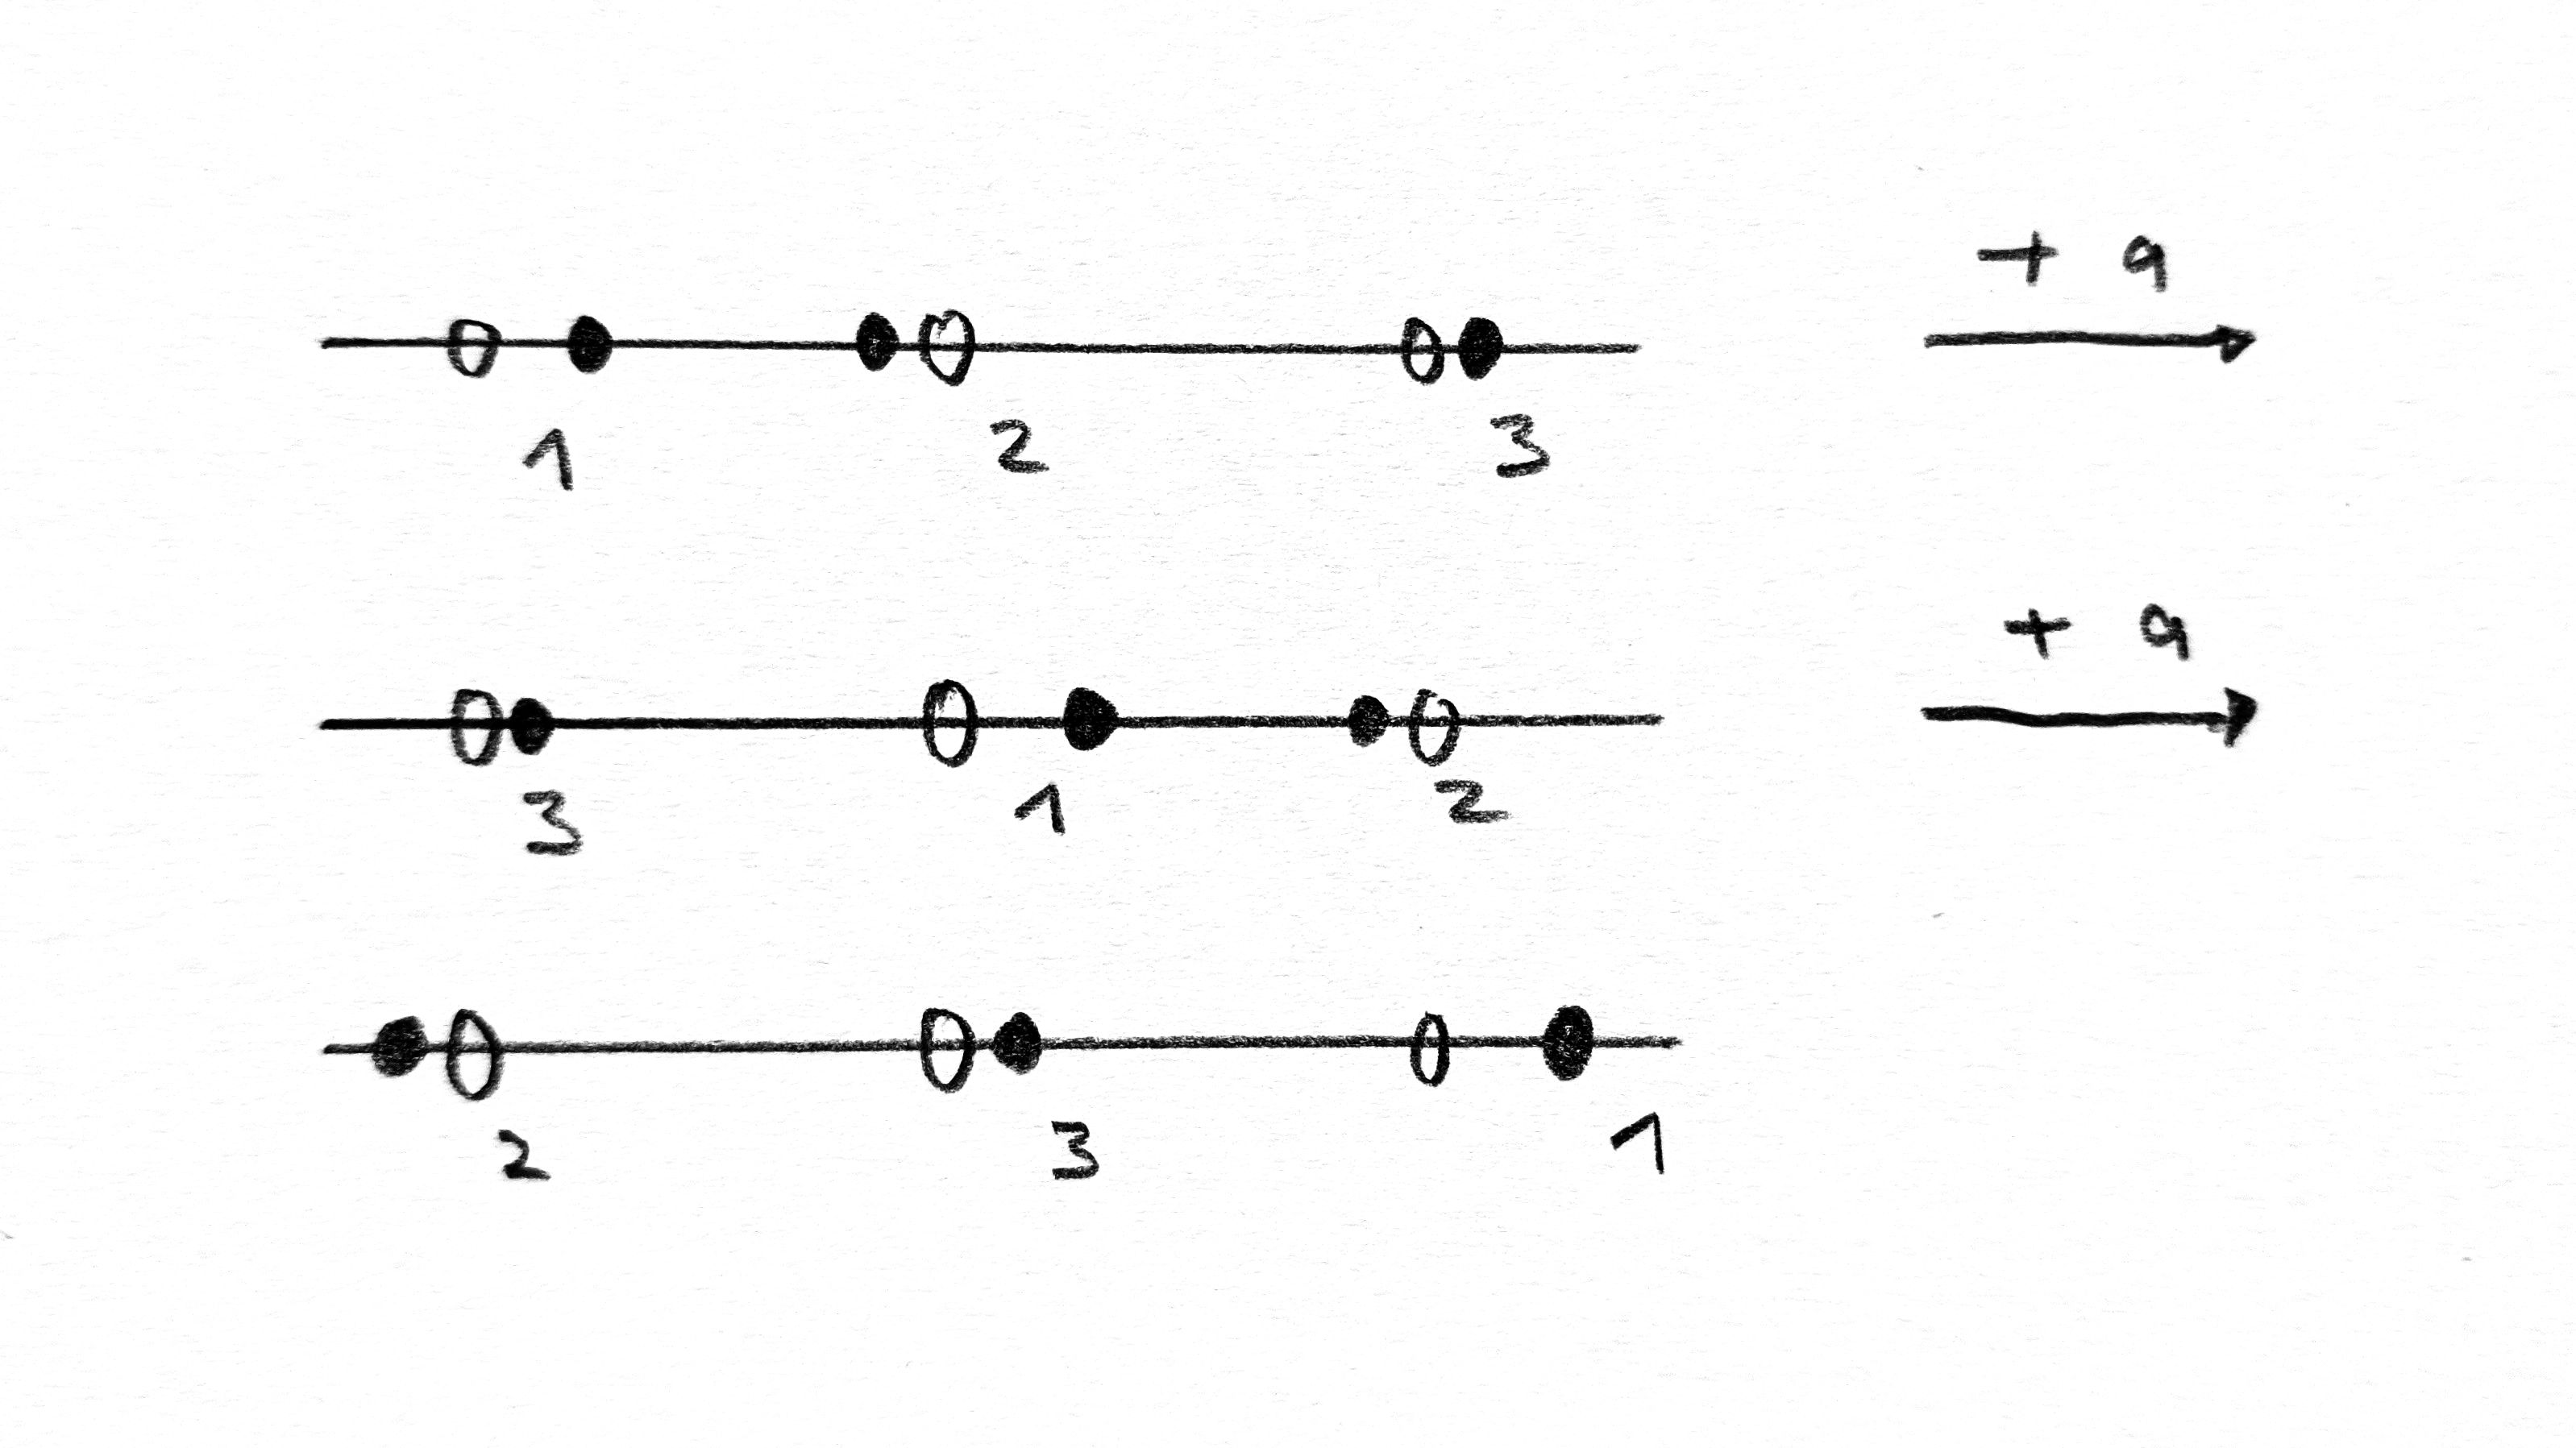
\includegraphics[width=.68\textwidth]{./sketches/permutation1.jpg}
	\caption{A linear chain with three atoms (bullets) displaced from their equilibrium position (open circels). With periodic boundary conditions, the consecutive translation by a lattice vector $a$ induces a permutation of the atoms,~i.\,e.,~$(1, 2 , 3) \to (3, 1, 2) \to (2, 3, 1)$.}
	\label{fig:translation.permutation}
\end{figure}

We can draw two important conclusions from Eq.\,\eqref{eq:translation.permutation} and \eqref{eq:inv.V}. First, the existence of the map $P_{\bf L}$ enables us to write every atomic coordinate ${\bf R}_I$ as
\begin{align}
	{\bf R}_I \equiv {\bf R}_{i {\bf L}} 
		= {\bf R}^0_i + {\bf U}_{i {\bf L}} + {\bf L}~,
	\label{eq:R_iL}
\end{align}
where ${\bf R}^0_i$ labels the position of an equivalent reference atom in the unit cell, ${\bf U}_{i {\bf L}}$ is the displacement of the atom from its equilibrium position, and $\bf L$ is a Bravais vector as before.
We can therefore split the index $I$ into a tuple $I = (i, {\bf L})$,~i.\,e.,~unit cell and lattice point labels.

Second, the harmonic force constants $\Phi_{I \alpha, J \beta}$ can be written as $\Phi_{i {\bf L} \alpha, j {\bf K} \beta}$~, where $\bf L$ and $\b K$ are the Bravais vectors belonging to $I$ and $J$, respectively. From the translational invariance of the potential, Eq.\,\eqref{eq:inv.V}, we see that the force constants have to fulfill
\begin{align}
	\Phi_{i {\bf L} + \b M \alpha, j {\bf K} + \b M \beta} 
		= \Phi_{i {\bf L} \alpha, j {\bf K} \beta}~,
	\label{eq:fc.sym.1}
\end{align}
where $\b M$ again denotes an arbitrary Bravais vector. Using this translational invariance, we can Fourier transform the dynamical matrix defined in Eq.\,\eqref{eq:D},
\begin{align}
	{\rm D}_{i \alpha, j \beta} (\b q) 
		= \sum_{\b L} {\rm e}^{- \im \b q \cdot \b L} {\rm D}_{i \b 0 \alpha, j \b L \beta}
	\label{eq:D(q)}
\end{align}
where we restrict the values of $\b q$ to reside in the first Brillouin zone, thereby transforming the $3N \times 3N$ matrix ${\rm D}_{IJ}$ to one $3n \times 3n$ matrix ${\rm D}_{ij} (\bf q)$ for each~$\b q$, where $n$ is the number of atoms in the primitive unit cell.

\subsubsection{Cyclic Boundary Conditions and Supercell Approximation}
In the previous section, we did not specify the system beyond requiring periodic boundary conditions, and implicitly assumed an infinite crystal in the limit $N \to \infty$ without boundaries. In practice we introduce Born-von Karman cyclic boundary conditions~\cite{born2013atomtheorie}, as already done in Sec.\,\ref{sec:theory.periodic.1} for the description of electronic states, but reintroduce them here in a slightly more general fashion.

We define the boundary conditions for the nuclear problem such that
\begin{align}
	\b R_I + S^i \b A_i = \b R_I \quad\text{for}\quad S^i \in \mathds{Z}~,
	\label{eq:sc.1}
\end{align}
where each ${\bf A}_i$ is a linear combination of the primitive basis vectors $\set{{\bf a}_i}$,
\begin{align}
{\bf A}_i = {\rm M}_{ij}^{\rm sc} {\bf a}_j\quad\text{with } {\rm M}_{ij}^{\rm sc} \in \mathds Z~,
\end{align}
and $\rm M^{\rm sc}$ is a non-singular matrix with integer elements. The space spanned by the $\set{{\bf A}_i}$ is parallelepiped of volume $V_{\rm sc} = N_{\rm sc} \, {\bf a}_1 \cdot ({\bf a}_2 \times {\bf a}_3)$, where $N_{\rm sc} = \det {\rm M}^{\rm sc}$ is the number of unit cells that fit into the enlarged cell, and $V_{\rm uc} = {\bf a}_1 \cdot ({\bf a}_2 \times {\bf a}_3)$ is the unit cell volume. This cell is therefore called \emph{supercell} and we define it such that its midpoint is located at the origin,~i.\,e.,~
\begin{align}
	\mathds V_{\rm sc}
		&= \set{{\bf X} = X^i {\bf A}_i : X^i \in {[-0.5, 0.5)_{\mathds R}}}~.
	\label{eq:supercell}
\end{align}
We therefore denote the matrix ${\rm M}^{\rm sc}$ as the \emph{supercell matrix}.
The vectors \mbox{$\b S = S^i \b A_i$} are the equivalent of the Bravais vectors $\b L$ in a superlattice described by $\set{ \b A_i }$ instead of $\set{ \b a_i}$.
The ideal, infinite crystal is obtained in the limit $N_{\rm sc} \rightarrow \infty$.
From Eq.\,\eqref{eq:sc.1} we see that the force constants become periodic functions in the superlattice,
\begin{align}
	\Phi_{i {\bf L} \alpha, j {\bf K} + \b S \beta} 
		= \Phi_{i {\bf L} \alpha, j {\bf K} \beta} \quad\text{for all}\quad \b S = S^i \b A_i~,
	\label{eq:fc.sym.2}
\end{align}
so that the dynamical matrix in Eq.\,\eqref{eq:D(q)} can be written as a sum over lattice points that are contained in the supercell only,
%\begin{align}
%	{\rm D}_{i \alpha, j \beta} (\b q) 
%		&= \sum_{\b L \in \mathds V_{\rm sc}} 
%			\left( 
%				{\rm e}^{- \im \b q \cdot \b L} {\rm D}_{i \b 0 \alpha, j \b L \beta}
%			+ \sum_{\b S \neq \b 0} {\rm e}^{- \im \b q \cdot (\b L + \b S)} {\rm D}_{i \b 0 \alpha, j \b L \beta}
%			\right)~.
%	\label{eq:D^S(q).1}
%\end{align}
\begin{align}
	{\rm D}_{i \alpha, j \beta} (\b q_{\bf m}) 	
		&= %\frac{N}{N_{\rm sc}} 
	\sum_{\b L \in \mathds V_{\rm sc}} {\rm e}^{- \im \b q_{\bf m} \cdot \b L} {\rm D}_{i \b 0 \alpha, j \b L \beta}~.
	\label{eq:D^S(q).2}
\end{align}
for $\b q_{\b m}$ that fulfill
\begin{align}
	{\bf q_{\b m}} \cdot {\bf A}_i	= 2 \pi m_i \quad\text{with}\quad m_i \in \mathds Z~.
	\label{eq:q.commensurate}
\end{align}
%the summands in the second sum of Eq.\,\eqref{eq:D^S(q).1} interfere constructively and yield a factor $\sum_{\b S}' = N / N_{\rm sc} - 1$. For all other $\b q$, the entire summand becomes negligible in the limit $N \to \infty$ when normalized to the supercell volume.
The $\b q_{\b m}$ that fulfill Eq.\,\eqref{eq:q.commensurate} are called \emph{commensurate} $\b q$-points, as they represent wave numbers that fit into the supercell.
In total there are $N_{\rm sc}$ non-equivalent values of $\bf q_{\b m}$ labelled by ${\bf m} = (m_1, m_2, m_3)$ that can be expressed in terms of the lattice vectors of the reciprocal supercell,
\begin{align}
{\bf B}^i 
= 2 \pi \varepsilon^{ijk} \frac{{\bf A}_j \times {\bf A}_k}{{\bf A}_1 \cdot ({\bf A}_2 \times {\bf A}_3)} ~,
%\label{eq:dft.Bloch.bi}
\end{align}
where $\varepsilon^{ijk}$ denotes the Levi-Civita symbol enforcing the correct ordering of $ijk$. The complete set of $\bf q$-values is
\begin{align}
{\bf q}_{\bf m} 
= \sum_{i=1}^3 m_i {\bf B}^i~,
\label{eq:q_m}
\end{align}
with $m_i \in \mathds Z$ such that $\b q_{\bf m}$ is an element of the first Brillouin zone of the direct lattice.
%For the set of commensurate $\b q$-points, the dynamical matrix is therefore given by
%\begin{align}
%{\rm D}_{i \alpha, j \beta} (\b q_{\bf m}) 	
%	&= %\frac{N}{N_{\rm sc}} 
%	\sum_{\b L \in \mathds V_{\rm sc}} {\rm e}^{- \im \b q_{\bf m} \cdot \b L} {\rm D}_{i \b 0 \alpha, j \b L \beta}~.
%	\label{eq:D^S(q).2}
%\end{align}


\subsubsection{Interpolation to non-commensurate q-points}
The definition of the dynamical matrix in Eq.\,\eqref{eq:D^S(q).2} was formulated for commensurate $\b q$-points $\set{\b q_{\b m}}$,~i.\,e.,~those given in terms of Eq.\,\eqref{eq:q_m}. Evaluating this expression at a non-commensurate value of $\b q$ will, in general, yield a non-hermitian matrix which cannot be used to extract physically sound information about the system. To obtain an \emph{approximated} dynamical matrix at any other, non-commensurate value of $\b q$ within the Brillouin zone, we define an \emph{extended supercell}, 
\begin{align}
	\mathds V_{\rm sc}^{\rm ext}
		&= \set{{\bf X} = X^i {\bf A}_i : X^i \in {[-0.5, 0.5 \boldsymbol{]}_{\mathds R}}}~,
	\label{eq:supercell.extended}
\end{align}
which also contains the lattice points at the positive boundary of the supercell as depicted by open circles in Fig.\,\ref{fig:sketch_supercells}.
\begin{figure}[t]
	\centering
	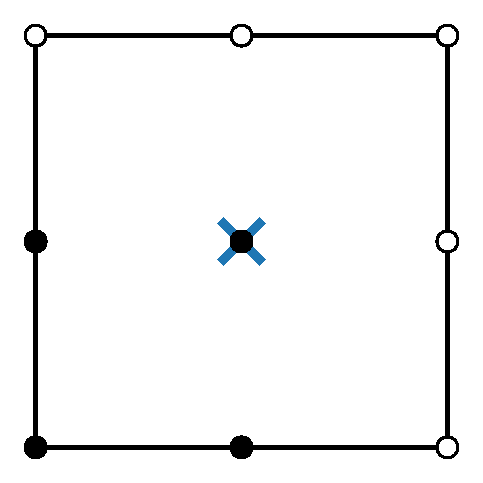
\includegraphics[width=.32\textwidth]{./sketches/2_sc.pdf}
	\hfill
	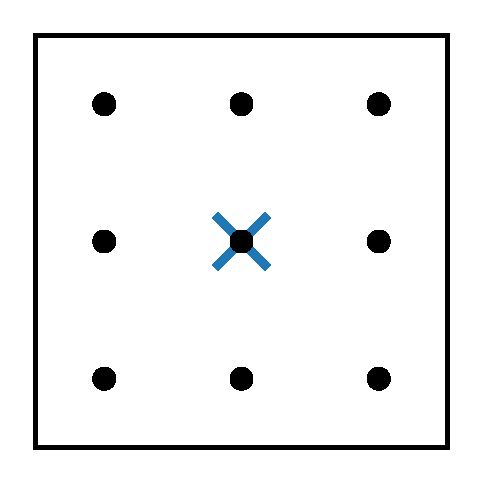
\includegraphics[width=.32\textwidth]{./sketches/3_sc.pdf}
	\hfill
	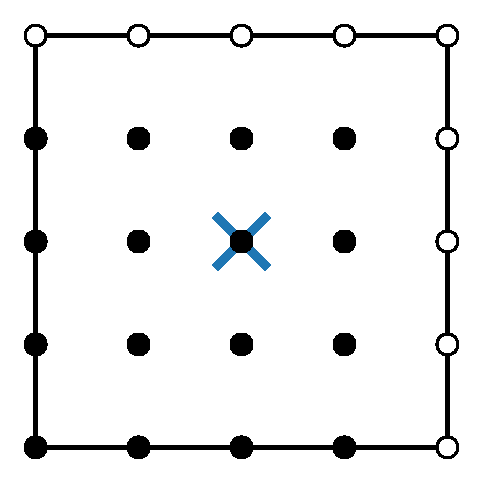
\includegraphics[width=.32\textwidth]{./sketches/4_sc.pdf}
	\caption{Depiction of square supercells with lattice points in the range $[-0.5 A, 0.5 A)$ (bullets $\bullet$), and extended lattice points at the supercell boundary (empty bullets $\circ$), where $A$ is the edge length of the supercell. Blue arrows denote the unit cell vectors, black arrows denote the supercell vectors.}
	\label{fig:sketch_supercells}
\end{figure}
These lattice points are included in the Fourier series with an appropriate weight $w_{\b L}$ that accounts for double counting of lattice points that are separated by a linear combination of supercell lattice vectors~\cite{Parlinski1997}. Furthermore, we use a minimal image convention (MIC) between the atoms $(i, \b 0)$ and $(j, \b L)$,~i.\,e.,~for each pair we use an equivalent lattice point $\b L'$ within the extended supercell which depends on $(i, j, \b L)$ such that
\begin{align}
	- \b R_{i \b 0 } + \b R_{j \b 0} + \b L' \in V_{\rm sc}^{\rm ext}~.
	\label{eq:L'}
\end{align}
In total we define
\begin{align}
	{\rm D}_{i \alpha, j \beta} (\b q) 	
		&= %\frac{N}{N_{\rm sc}} 
		\sum_{\b L \in \mathds V_{\rm sc}^{\rm ext}} 
			w_{\b L}
		{\rm e}^{- \im \b q \cdot \b L'} {\rm D}_{i \b 0 \alpha, j \b L \beta}~.
	\label{eq:D_Parlinski}
\end{align}
We note that the dynamical matrix elements defined by Eq.\,\eqref{eq:D_Parlinski} differ from the ones found in Ref.~\cite{Parlinski1997} by a phase factor ${\rm e}^{\im \b q \cdot (\b R_i^0 - \b R_j^0)}$, which is typical when the discussion is performed from a lattice-wave ansatz to solve the equations of motion~\cite[p. 298]{BornHuang}.

For each $\b q$, ${\rm D} (\b q)$ is a hermitian $3n \times 3n$ matrix in the indices $(i \alpha, j \beta)$ and will therefore yield $3n$ real eigenvalues and $3n$ complex, orthogonal eigenvectors, which denote in accordance with Eq.\,\eqref{eq:sum_D_IJ}
\begin{align}
\sum_{j \beta} {\rm D}_{i \alpha, j \beta} (\b q) e_{j \beta} (\b q , b)
= \omega^2 \, (\b q, b) e_{i \alpha} (\b q , b)~,
\label{eq:D_ij(q)w}
\end{align}
where the \emph{band index} $b$ is used to discern the $3n$ \emph{branches} at each $\b q$. Using the combined index $s = (\b q, b)$, the notation becomes similar to the non-periodic case with $3N_{\rm sc} N_{\rm uc}$ degrees of freedom, only that the eigenvectors $\b e_{s = (\b q, n)}$ can be complex valued instead of strictly real.
\REM{This is Born conventions. Togo and Parlinski use extra phase factor ${\rm e}^{\im \b q \cdot (\b R_i^0 - \b R_j^0)}$ that alters the eigenvectors but not the frequencies.}

\subsubsection{Ledermann's Theorem}

%As we will be interested in the eigenvalues and eigenvectors of the dynamical matrices $\rm D ({\b q})$, the prefactor $N/N_{\rm sc}$ can be neglected in the following.

\REM{for $\b q = \b q_{\b m}$ D is exact up to boundary effects (?!), nevertheless one can interpolate -> Fourier interpolation}
\REM{Alternative: Use effective cutoff of $\Phi$}
\REM{Effective cutoff -> effect on spectrum, Maradudin, Ledermann}

% Equation~\eqref{eq:D^S(q).2} will in general not be hermitian in $(i \alpha, j \beta)$

\subsubsection{Finite Differences}
The force constants can be obtained from first-order derivatives of the potential-energy surface,~i.\,e.,~the forces, by rewriting the second derivative in terms of a finite difference expression,
\begin{align}
	\Phi_{I \alpha, J \beta}
		= \left.\frac{\partial^{2} \mathcal{V}(\mathbf{R})}{\partial R_{I}^{\alpha} \partial R_{J}^{\beta}}\right|_{\mathbf{R}^{0}}
		= - \frac{\partial}{\partial R_I^\alpha} F_{J, \beta}
		= - \lim_{\epsilon \to 0}
			\frac{F_{J, \beta} (\set{\b R': R^{\prime \beta}_I = R^{\beta}_I + \epsilon )}}{\epsilon}
		~.
\label{eq:FC2_finite}
\end{align}
In practice, atom $J$ is displaced by a small but finite displacement $\epsilon$ in the direction $\beta$, and the force on all other atoms is recorded. By performing the displacement in all $3N$ degrees of freedom, the $3N \times 3N$ forces can be arranges in a matrix $F_{[3N \times 3N]}$, and the displacements can be arranged in a matrix $U_{[3N \times 3N]} = \epsilon \mathds 1_{[3N \times 3N]}$. The $3N \times 3N$ force-constants matrix $\Phi$ is obtained by the trivial matrix inversion
\begin{align}
F &= - H U = - \epsilon \Phi \mathds 1\\
\implies
\Phi &= - \frac{1}{\epsilon} F \mathds 1~.
\end{align}
%\begin{align}
%	F &= - H U \\
%	\implies
%	H &= - U^{+} F \\
%	F &= \begin{pmatrix} \b F_1, & \cdots, & \b F_{3N} \end{pmatrix}
%\end{align}
If $M > 3N$ displacements are used,~e.\,g.,~because positive and negative displacements $\pm \epsilon$ are used, the force constants can be obtained by solving an overdetermined linear equation of the kind
\begin{align}
	F_{[3N \times M]} &= - \Phi_{[3N \times 3N]} U_{[3N \times M]} \\
	\implies
	\Phi &= - U^{+} F~,
%	F &= \begin{pmatrix} \b F_1, & \cdots, & \b F_{3N} \end{pmatrix}
\end{align}
where $U^{+}$ denotes the Moore-Penrose pseudo inverse of the displacement matrix $U$~\CITE{pseudoinverse}.
\CITE{Parlinski, Togo}

In practice, the number of required force calculations can be reduced by considering the spacegroup symmetry of the crystal. This can be achieved in two ways: First, the symmetry can be used to identify the set of inequivalent displacements from which all other forces can be reconstructed. Second, the symmetry can be used to reduce the forceconstant matrix to an irreducible basis.

\REM{Symmetry: 2 ways: i) construct full $F$ from a reduced set of displacements, ii) reduce $H$ to reduces/irreducible representation like original Parlinski article.}

\subsection{Harmonic Sampling}

\subsection{Molecular Dynamics}
The classical limit of the nuclear Schr\"odinger equation~\eqref{eq:BOSE} is usually performed by writing the nuclear wavefunction $\chi_s ({\bf R}, t)$ in terms of a real amplitude $A_s({\bf R}, t)$ and a \emph{classical action function} $S_s({\bf R}, t)$~\cite{Dirac1981,Landau2013,Marx2009}
\begin{align}
	\chi_s({\bf R}, t) = A_s({\bf R}, t) \, {\rm e}^{\frac{\im}{\hbar} S_s({\bf R}, t)}~.
	\label{eq:class.1}
\end{align}
The Schr\"odinger equation then yields a set of differential equations for $A_s$ and $S_s$ that, in the limit $\hbar \to 0$, go over to a \emph{Hamilton-Jacobi} equation for $S_s$,~i.\,e.,~
\begin{align}
  \frac{\partial S_s}{\partial t} + \mathcal H \left({\bf R}, {\bf P}\right)
  = 0~,
  \label{eq:HamiltonJacobi}
\end{align}
where ${\bf P} = ({\bf P}_1, \ldots) \equiv ({\bf \nabla}_1 S_s, \ldots)$ denotes the conjugate momenta and $\mathcal H$ is the \emph{classical} Hamilton function corresponding the to the operator in Eq.\,\eqref{eq:BOSE}, from which the equations of motion for the nuclei can be obtained:
\begin{align}
  \dot{{\bf P}}_I 
    = -\frac{\partial \mathcal H}{\partial {\bf R}_I}
    \quad\implies\quad M_I \ddot{\bf R}_I
    = -\frac{\partial \mathcal V}{\partial {\bf R}_I}~.
    % \equiv - {\bf F}_I~.
\end{align}
The negative gradient of the Born-Oppenheimer potential, 
$-\partial \mathcal V / \partial {\bf R}_I$ is the force ${\bf F}_I$ acting on atom $I$ which can be obtained via the Hellmann-Feynmann theorem,~cf.~Sec.\,\ref{sec:HellmannFeynman}.

An alternative viewpoint that is more instructive can be taken by invoking the \emph{Ehrenfest theorem}~\cite{Ehrenfest1927,Basdevant2007}. The statement is that
\begin{align}
  \frac{\d}{\d t} \left\langle {\bf P}_I \right\rangle_{\chi_s}
    = \left\langle
      - \frac{\partial \mathcal{V}}{\partial {\bf R}_I}
    \right\rangle_{\chi_s}~,
  \label{eq:ehrenfest.de1}
\end{align}
where $\langle \cdot \rangle_{\chi_s}$ denotes an expectation value taken with respect to the state $\chi_s$. This expression differs only slightly from the classical counterpart, which would read
\begin{align}
\frac{\d}{\d t} \left\langle {\bf P}_I \right\rangle
= \left.
- \frac{\partial \mathcal{V}}{\partial {\bf R}_I}
\right\vert_{{\bf R} = \langle {\bf R} \rangle}~.
\label{eq:ehrenfest.de2}
\end{align}
The difference comes from the fact that, in general,
\begin{align}
  \delta f  \equiv 
  f \bm ( \langle x \rangle \bm{)} 
  - 
  \bm{\langle} f (x) \bm{\rangle}
  \neq 0
  ~,
  \label{eq:ehrenfest.delta1}
\end{align}
where $x = {\bf R}_I$ denotes the space coordinate for notional simplicity, $f$ is some function of the observable $x$, and $\delta f$ measures the difference between the classical and the quantum expectation value. Ehrenfest's argument is that this difference becomes negligible when the state is sufficiently peaked around some value $x_0$. Expanding $f$ around the expectation value of $x$, $x_0 \equiv \langle x \rangle$, we have
\begin{align}
  f(x) = f \bm ( \langle x \rangle \bm{)}  
    + (x - \langle x \rangle) \, f' \bm ( \langle x \rangle \bm{)}
    + \frac{1}{2} (x - \langle x \rangle)^2 \, f'' \bm ( \langle x \rangle \bm{)}
    + \cdots~.
  \label{eq:ehrenfest.f2}
\end{align}
It follows that the $f'$ term vanishes when the expectation value is taken, and
\begin{align}
\langle f(x) \rangle 
  = f \bm ( \langle x \rangle \bm{)}  
    + \frac{1}{2} \Delta x^2 f'' \bm ( \langle x \rangle \bm{)}
    + \cdots~,
\label{eq:ehrenfest.f3}
\end{align}
where $\Delta x^2 = \bm{\langle} (x - \langle x \rangle)^2 \bm{\rangle}$ measures the variance of the underlying distribution,~i.\,e.~the width of the wavepacket. The relative error between the classical and quantum expectation value is readily computed to be
\begin{align}
  \left\lvert \frac{\delta f}{f \bm ( \langle x \rangle \bm{)}} \right\rvert
  = \frac{1}{2} \Delta x^2 \left\lvert \frac{f'' \bm ( \langle x \rangle \bm{)}}{f \bm ( \langle x \rangle \bm{)}} \right\rvert
+ \mathcal{O}(\Delta x^3)~.
  \label{eq:ehrenfest.delta2}
\end{align}
This estimation holds in general for any observable $f$.
By crudely estimating the dimension of the wavepacket in terms of the thermal de Broglie-wavelength, we find
\begin{align}
  \Delta x^2 
    \sim \left( \frac{h}{P} \right)^2
    \sim \frac{h^2}{MT}~,
  \label{eq:ehrenfest:dimension}
\end{align}
which gives support to the intuitive assumption that we can expect the classical limit to work better the heavier the atoms and the higher the temperature.
Let us now set $f(x) \hat = -\partial \mathcal V / \partial {\bf R}_I$, then another important conclusion can be drawn from Eq.\,\eqref{eq:ehrenfest.delta2}: For a harmonic potential $\mathcal V ({\bf R}) = \mathcal V^{(2)} ({\bf R})$, where derivatives higher than second order vanish, the classical and quantum mechanical expectation values \emph{always coincide}. The quantum mechanical expectation value of position will therefore evolve in the same time-periodic fashion as a classical particle in a harmonic well.

\REM{this approach can only be validated by computing observables and compare the results. One can safely say that this approach has been used successfully in a plethora of studies, while additional care must be taken at low temperature and/or systems with light atoms, especially hydrogen-bonded systems~\CITE{MD-Review?,MarklandCeriotti,Litman,pHexperiment}.}

\subsubsection{Thermodynamic Ensembles and Thermostats}
\subsubsection{Finite Temperature Equations of State and Lattice Expansion}
\subsubsection{Mode Projection}
\subsubsection{Approximative Anharmonic Methods}

\subsection{Heat Transport}
\subsubsection{Fluctuation Dissipation Theorem}
\subsubsection{Green and Kubo}
\subsubsection{Ab initio Virial Heat Flux}
\subsubsection{Ab initio Green Kubo}

\chapter{Screening Materials for Anharmonicity}
\section{Anharmonicity Measure}
\section{Screening Material Space}
\subsubsection{Literature Review}
\subsection{Candidate Materials}

\chapter{Thermal Conductivities for Strongly Anharmonic Compounds}
\section{Overview: Results of Dataset}
\section{Discussion}
\subsubsection{Relation to Anharmonicity}
\subsubsection{Dynamical Effects}

\chapter{Conclusion}

\chapter{Outlook}

\bibliography{references}
\bibliographystyle{unsrt}

\appendix
\chapter{Bloch Theorem and Brillouin Zone}
\epigraph{\singlespacing \it ``The idea of periodicity in the reciprocal space is useless but, I think, harmless.''}{Paul Gartner}
\section{Bloch Theorem}
\label{sec:BlochTheorem}
The Schr\"odinger equation in 1d reads
\begin{align}
	\hat H \psi (x) = \left( - \frac{\nabla^2}{2m} + V(x) \right) \psi (x) = E \psi (x)~.
	\label{eq:app.bloch.se}
\end{align}
In a periodic potential,
\begin{align}
	V(x + a) = V(x)~,
	\label{eq:app.bloch.potential}
\end{align}
the periodicity can be expressed by stating that the translation operator $\hat T_a$ defined by its action,
\begin{align}
	\hat T_a f(x) = f(x + a)~,
	\label{eq:app.bloch.Ta}
\end{align}
commutes with the Hamiltonian,
\begin{align}
	\left[ \hat H , \hat T_a\right] = 0~.
	\label{eq:app.bloch.commute}
\end{align}
The eigenstates $\psi (x)$ of $\hat H$ are therefore also eigenstates of $\hat T_a$~\cite{Basdevant2000}. The translation operator is unitary, $\D{\hat T}_a = \hat{T}_a^{-1}$, but not hermitian. The eigenvalues $\lambda$ associated with $\hat T_a$ are thus complex numbers. By definition, one has \mbox{$\psi ( x + na ) = \lambda^n \psi(x)$}. Requiring bounded solutions, $\lim_{x \rightarrow \infty} \lvert \psi (x) \rvert < \infty$, imposes the condition $\lvert \lambda \rvert = 1$.
The function $\psi$ can therefore be written as
\begin{align}
	\psi (x) = c(x) u(x)~,
\end{align}
with a real, periodic function
\begin{align}
	u: \mathds R \rightarrow \mathds R
	\quad\text{with}\quad u(x + a) = u(x)~,
\end{align}
and a complex function of unit modulus,
\begin{align}
	c: \mathds R \rightarrow \mathds C
	\quad\text{with}\quad \left\lvert c(x) \right\rvert = 1~.
	\label{eq:app.bloch.c1}
\end{align}
We label each possible solution by the number $k$, then
\begin{align}
	c_k (x) = {\rm e}^{\im k x}
	%% don't impose uniqeness here
	%\quad\text{with}\quad k \in \left[0, \frac{2 \pi}{a} \right)
	\label{eq:app.bloch.c2}
\end{align}
% is a unique map from the domain $x \in [0, a)$ to the complex unit circle $\set{z \in \mathds C : \lvert z \rvert = 1}$. 
is a map from the domain $x \in \mathds R$ to the complex unit circle $\set{z \in \mathds C : \lvert z \rvert = 1}$. 
It then holds that $\hat T_a \psi_k (x) = {\rm e}^{\im k a} \psi(x)$,~i.\,e.,~$\psi_k$ is an eigenfunction of $\hat T_a$ with eigenvalue $\lambda = {\rm e}^{\im k a}$. We formulate the
\begin{thm}[Bloch]
	Solutions to the Schr\"odinger equation~\eqref{eq:app.bloch.se} with a periodic potential of periodicity $a$ are of the form
	\begin{align*}
		\psi_k (x) = {\rm e}^{\im k x} u_k (x)~,
	\end{align*}
	with a real, periodic function $u_k$.
%	 for each $k$ in the first Brillouin zone,
%	\begin{align*}
%		k \in \left[0, \frac{2 \pi}{a} \right)~.
%	\end{align*}
\end{thm}
The theorem is trivially extended to the 3d case by using the multiplication rule
\begin{align}
	\hat{T}_{{\bf a} + {\bf b}} f({\bf x}) = \hat{T}_{\bf a} \hat{T}_{\bf b} f({\bf x}) \equiv f({\bf x} + {\bf a} + {\bf b})~.
\end{align}
A more rigorous proof in terms of representation theory can be found,~e.\,g.,~in~\cite{Dresselhaus2007}.

\section{Brillouin Zone}
\label{sec:BrillouinZone}
We have not yet specified the range of the quantum number $k$. This can be done by requiring the complex function $c_k$ defined in Eq.\,\eqref{eq:app.bloch.c2} to map the interval $x \in [0, a)$ \emph{exactly once} to the unit circle so that $k$ is a \emph{unique} label for the eigenvalues ${\rm e}^{\im k a}$ of the translation operator $\hat T_a$.
We therefore define the
\begin{align}
	\text{Brillouin zone} = \set{k : k \in \left[ - \frac{\pi}{a}, \frac{\pi}{a}\right)}~.
\end{align}
For a wavefunction belonging to $k' = k + G$, where $G$ is an integer multiple of the the reciprocal lattice vector $b = 2\pi / a$, we would find
\begin{align}
	\hat T_a \psi_{k + G} (x) = {\rm e}^{\im k a} \psi_{k + G} (x)~.
\end{align}
They are therefore indistinguishable by the translation operator and we define $\psi_k$ and $\psi_{k+G}$ to be the same function,
\begin{align}
	\psi_k (x) = \psi_{k + G} (x)~.
\end{align}
This is sometimes termed ``periodicity of Bloch functions in reciprocal space''.

\chapter{Born-von Karman Supercell}
To ensure normalizability of the functions $\psi_{{\bf k}l}$, one additionally imposes the \emph{Born-von Karman boundary conditions}
\begin{align}
\psi_{{\bf k}l} ({\bf x} + {\bf A}_i) 
= \psi_{{\bf k}l} ({\bf x})
%\label{eq:dft.Bloch.4}
\end{align}
where each ${\bf A}_i$ is a linear combination of the primitive basis vectors $\set{{\bf a}_i}$,
\begin{align}
{\bf A}_i = S_i^{~j} {\bf a}_j\quad\text{with } S_i^{~j} \in \mathds Z~,
\end{align}
where $S$ is a non-singular matrix with integer elements. The space spanned by the $\set{{\bf A}_i}$ is parallelepiped of volume $V = N \, {\bf a}_1 \cdot ({\bf a}_2 \times {\bf a}_3)$, where $N = \det S$ is the number of unit cells that fit into the enlarged cell. This cell is therefore often called \emph{supercell}, and the matrix $S$ is denoted as a \emph{supercell matrix}.
With the Born-von Karman boundary conditions, the domain of all functions and functionals appearing in the Kohn-Sham equations become restricted to the supercell. The ideal, infinite crystal is obtained in the limit $N \rightarrow \infty$.
Using the periodic boundary condition expressed by Eq.\,\eqref{eq:dft.Bloch.4} in the Bloch functions given by Eq.\,\eqref{eq:dft.Bloch.2}, and the periodicity of the functions $u_{{\bf k} l}$, one finds that
\begin{align}
%	{\rm e}^{\im {\bf k} \cdot ({\bf x} + N_i {\bf a}_i)} u_{{\bf k} l} ({\bf x})
%		&= {\rm e}^{\im {\bf k} \cdot {\bf x}} u_{{\bf k} l} ({\bf x}) \nonumber \\
%	\implies
%		{\rm e}^{\im {\bf k} \cdot  N_i {\bf a}_i} 
%			&= 1 \nonumber \\
%	\implies
{\bf k} \cdot {\bf A}_i
&= 2 \pi m_i\quad\text{with } m_i \in \mathds N \text{ such that } 
\forall i: {\bf k} \cdot {\bf a}_i \leq 2 \pi~.
%\label{eq:dft.Bloch.5}
\end{align}
In total there are $N$ permissible values of $\bf k$ labelled by ${\bf m} = (m_1, m_2, m_3)$ that can be expressed in terms of the \emph{reciprocal lattice vectors}~\cite{Sands2002}
\begin{align}
{\bf B}^i 
= 2 \pi \varepsilon^{ijk} \frac{{\bf A}_j \times {\bf A}_k}{{\bf A}_1 \cdot ({\bf A}_2 \times {\bf A}_3)} ~,
%\label{eq:dft.Bloch.bi}
\end{align}
where $\varepsilon^{ijk}$ denotes the Levi-Civita symbol enforcing the correct ordering of $ijk$. The complete set of $\bf k$-values is
\begin{align}
{\bf k}_{\bf m} 
= \sum_{i=1}^3 m_i {\bf B}^i~.
%\label{eq:dft.Bloch.k_m}
\end{align}
The values of $\bf k$ given by Eq.\,\eqref{eq:dft.Bloch.k_m} are those sampled in real-space simulation in a box of the given size,~i.\,e.,~the \emph{Born-von Karman cell}.

\chapter{Finite Differences Force Constants}
The force constants $\Phi$ can be obtained from first-order derivatives of the potential-energy surface,~i.\,e.,~the forces, by rewriting the second derivative in terms of a finite difference expression,
\begin{align}
\Phi_{I \alpha, J \beta}
= \left.\frac{\partial^{2} \mathcal{V}(\mathbf{R})}{\partial R_{I}^{\alpha} \partial R_{J}^{\beta}}\right|_{\mathbf{R}^{0}}
= - \frac{\partial}{\partial R_I^\alpha} F_{J, \beta}
= - \lim_{\epsilon \to 0}
\frac{F_{J, \beta} (\set{\b R': R^{\prime \alpha}_I = R^{0, \alpha}_I + \epsilon )}}{\epsilon}
~.
\label{eq:FC2_finite}
\end{align}
In practice, atom $I$ is displaced by a small but finite displacement $\epsilon$ in the direction $\alpha$, and the force on all other atoms is recorded. By performing the displacement in all $3N$ degrees of freedom, the $3N \times 3N$ forces can be arranged in a matrix ${\rm F}_{[3N \times 3N]}$, and the displacements can be arranged in a matrix ${\rm U}_{[3N \times 3N]} = \epsilon \mathds 1_{[3N \times 3N]}$. The $3N \times 3N$ force-constants matrix $\Phi$ is obtained by the trivial matrix multiplication
\begin{align}
{\rm F }
&= - \Phi {\rm U} 
= - \epsilon \Phi \mathds 1
\label{eq:finite.diff.1}
\\
\implies
\Phi &= - \frac{1}{\epsilon} {\rm F} \mathds 1~.
\end{align}
%\begin{align}
%	F &= - H U \\
%	\implies
%	H &= - U^{+} F \\
%	F &= \begin{pmatrix} \b F_1, & \cdots, & \b F_{3N} \end{pmatrix}
%\end{align}
If $M > 3N$ displacements are used,~e.\,g.,~because positive and negative displacements $\pm \epsilon$ are used, the force constants can be obtained by solving an overdetermined linear equation of the kind
\begin{align}
{\rm F}_{[3N \times M]} &= - \Phi_{[3N \times 3N]} {\rm U}_{[3N \times M]} \\
\implies
\Phi &= - {\rm F} {\rm U}^{+}~,
\label{eq:phi.pseudo.1}
\end{align}
where ${\rm U}^{+}$ denotes the Moore-Penrose pseudo inverse of the displacement matrix $\rm U$~\cite{Penrose1955,Parlinski1997}.

\newthought{The number of required force calculations} can be reduced by considering the spacegroup symmetry of the crystal. This can be achieved in two ways: First, the symmetry can be used to identify the set of inequivalent displacements from which all other forces can be constructed by the following argument: We define the representation $\Gamma^g$ of a symmetry operation $g$ by its action on the atomic coordinates $\set{\b R_I = \b R_I^0 + \b U_I}$ as
\begin{align}
\b R_I^{g} &\equiv {\Gamma}^g (\b R_I) = { P}^g_{IJ} \b R^0_J + { M}^g \b U_I~,
\label{eq:sym.RI'}
\end{align}	
where $P^g_{IJ}$ is the permutation that relates the reference positions of atom $I$ and atom $J$, and $M^g$ is an orthogonal matrix representing the rotation (or inversion) of the respective displacement. 
\begin{marginfigure}
	\centering
	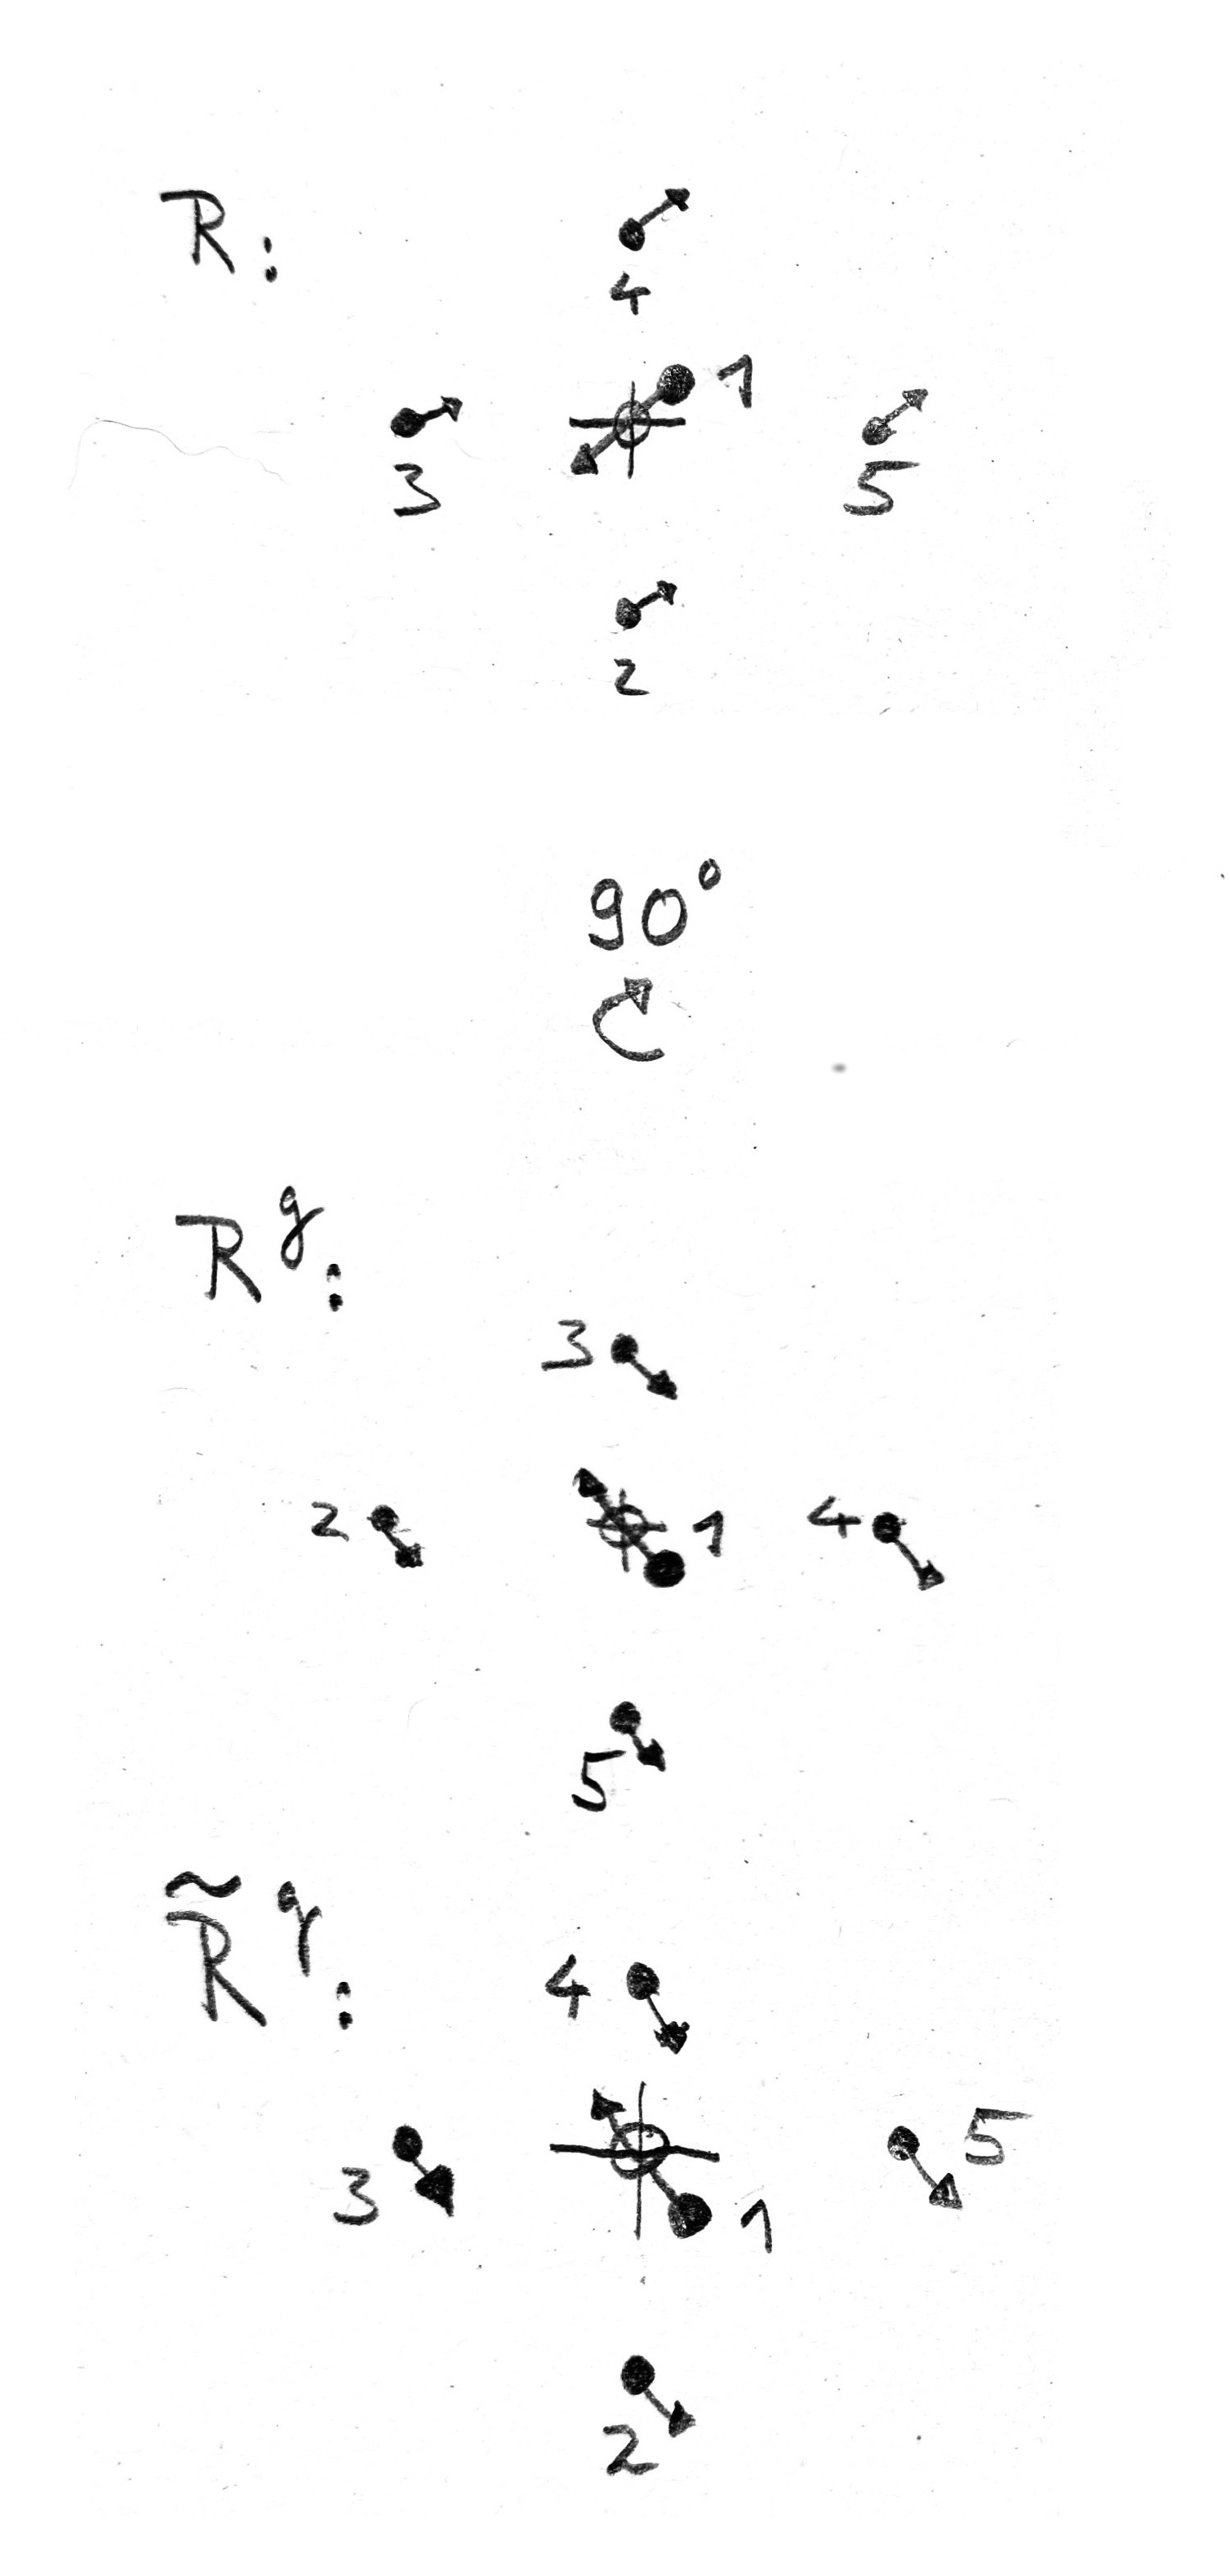
\includegraphics[width=\textwidth]{./data/sketches/symop.jpg}
	\caption{The configurations $\b R$, $\b R^g$, and $\tilde{\b R}^g$ obtained from the symmetry operation $g=\text{90 degrees rotation}$ for a two-dimensional system with five atoms. Arrows indicate the force at each atom.}
	\label{fig:symmetry.1}
\end{marginfigure}
As depicted in Fig.~\ref{fig:symmetry.1}, the forces on each atom in the rotated system $\b R^g = \set{\b R^g_I}$ are obtained by co-rotating the forces in the initial configuration $\b R = \set{\b R_I}$ as
\begin{align}
\b F_I (\b R^g) &= {M}^g \b F_I (\b R)~,
\label{eq:sym.Fp}
\end{align}
i.\,e.,~the forces transform as the displacements $\b U_I$. Let us now define a new configuration $\tilde{\b R}^g$ where just the displacements $\b U_I$ are rotated according to $g$. This can be achieved by rotating the entire system according Eq.\,\eqref{eq:sym.RI'} and applying the inverse permutation $P^{g-1}$,~i.\,e.,
\begin{align}
\tilde{\b R}_I^g 
&= P^{g-1}_{IJ} \b R_I^g 
\stackrel{\eqref{eq:sym.RI'}}{=} \b R^0_I + {\rm M}^g P^{g-1}_{IJ} \b U_J~.
\end{align}
It follows that the force on atom $I$ in the new configuration $\tilde{\b R}^g$ is related to the force in the rotated system $\b R^g$ by this inverse permutation, so that
\begin{align}
\b F_I (\tilde{\b R}^g) 
&= {P}^{g-1}_{IJ} \b F_J (\b R^g) 
= {M}^g  {P}^{g-1}_{IJ} \b F_J (\b R)~.
\label{eq:sym.Ftilde}
\end{align}
By means of this equation, the set of forces obtained for a configuration $\set{\b R_I = \b R_I^0 + \b U_I}$ can be used to generate a set of forces for each symmetrically equivalent configuration $\set{\tilde{\b R}_I^g = \b R_I^0 + {\rm M}^g P^{g-1}_{IJ} \b U_J}$, where $g$ are spacegroup elements.

A complementary approach is to use the symmetry elements $\set{g}$ to reduce the forceconstant matrix to an irreducible basis,
\begin{align}
\Phi 
= \sum_{i=1}^{D} p_i \tilde{\Phi}_i~,
\label{eq:sym.Phi.irrep.1}
\end{align}
where the $\tilde{\Phi}_i$ are \emph{solely} determined by the space group elements $\set{g}$ and analytical properties of the forceconstants, and only the \emph{irreducible components} $p_i$ are system dependent. The pseudoinverse procedure given in Eq.\,\eqref{eq:phi.pseudo.1} then only has to be performed for the $D$ parameters $p_i$~\cite{Parlinski1997}. This procedure can drastically reduce the number of free parameters in the forceconstant matrix. For example, in a $4\times4\times4$ bcc lattice with 128 atoms, $\Phi$ is a matrix with $(3 \cdot 128)^2 = 147456$ elements. However, there are only $D=11$ irreducible parameters $p_i$ that need to be determined~\cite{Hellman2013}.

\TODO{Add the theory for symmetry reduction}

\chapter{Linear Response Distribution Function}
\label{app:lr.f}
To solve for $\Delta f(t)$ defined in Eq.\,\eqref{eq:lr.df.2}, we introduce a shorthand notation such that
\begin{align}
\frac{\d \Delta f}{\d t} = -\im L \Delta f(t) - \im \Delta L (t) f^0~,
\label{eq:lr.df.3}
\end{align}
where the Liouville operator $L^0$ is defined by
\begin{align}
	\im L^0 g = \set{g, H^0}~,
	\label{eq:app.lr.L}
\end{align}
and similarly
\begin{align}
	\im \Delta L (t) g = \set{g, H'(t)}~.
	\label{eq:app.lr.L'}
\end{align}
Equation~\eqref{eq:lr.df.3} is a first order linear differential equation of the form
\begin{align}
	\frac{\d y}{\d t} + p(t) y = q(t)~,
	\label{eq:app.lr.dgl.1}
\end{align}
which is straightforward to solve by using an integrating factor as follows: We identify $y = \Delta f$, $p(t) = \im L^0$, and $q(t) = - \im \Delta L (t) f^0$. Following Ref.~\cite[p.\,68]{Lomen1986}, we define the integrating factor \mbox{$\rho (t) = \exp(\int \d t \, p (t)) = \exp (\im L^0 t)$}, multiply Eq.\,\eqref{eq:lr.dgl.1} with $\rho (t)$, and use that \mbox{$\frac{\d}{\d t} \, \rho(t) = \rho(t) p(t)$} to obtain
$$
\frac{\d}{\d t} (\rho (t) y) = \rho(t) q(t)~.
$$
This gets integrated to
$$
\rho(t) y = \int_{-\infty}^t \d t' \, \rho(t') q(t')
$$
under the boundary condition $y (t \to -\infty) = 0$. In total we obtain
\begin{align}
  y(t) 
    &= \rho^{-1} (t) \int_{-\infty}^t \d t' \, \rho(t') q(t')~, \\
  \implies
  \Delta f(t) 
    &= - {\rm e}^{- \im L^0 t}  \int_{-\infty}^t \d t' \, {\rm e}^{\im L^0 t'} \im \Delta L (t') f^0~.
\end{align}

\chapter{Explicit Formulas}
\section{Harmonic Approximation}
\label{app:ha.formulas}
In Sec.\,\ref{sec:dynmat.periodic}, we introduced the shorthand notation $s=(b, \b q)$, $-s=(b, -\b q)$ to write brief formulas. We give the explicit form of these formulas here.

\newthought{The normal mode coordinates} in the periodic case in terms of complex amplitudes $a^{(\dagger)}_b (\b q)$ read
\begin{subequations}
	\label{eq:u_b(q).amplitudes}
	\begin{align}
	u_b (\b q)
	&=   \frac{1}{\sqrt{2 \omega_b (\b q)}} \left[ \D a_b (- \b q) + \fD a_b (\b q)  \right] \\
	p_b (\b q)
	&= \im \sqrt{\frac{\omega_b (\b q)}{2}} \left[ \D a_b (- \b q) - \fD a_b (\b q)  \right]
	\end{align}
	\end{subequations}
	The inverse relation is given by
	\begin{subequations}
		\label{eq:a(q)}
		\begin{align}
		a_b (\b q)
		&= \sqrt{\frac{\omega_b (\b q)}{2}} u_b (\b q) + \frac{\im}{\sqrt{2 \omega_b (\b q)}} p_b (\b q) \\
		a^\dagger_b (-  \b q)
		&= \sqrt{\frac{\omega_b (\b q)}{2}} u_b (\b q) - \frac{\im}{\sqrt{2 \omega_b (\b q)}} p_b (\b q)
		\end{align}
		\end{subequations}
		The displacements are recovered by
		\begin{align}
		\b u_{i \b L}
		&= \frac{1}{\sqrt{N_{\b q}}} \sum_{b \b q} {\rm e}^{\im  \b q \cdot \b R^0_{i \b L}} \, \b e^\ast_{b i} (\b q) \fD u_b (\b q)
		\label{eq:u_iL}
		% \\
		% \b p_{i \b L}
		% &= \frac{1}{\sqrt{N_{\b q}}} \sum_{b \b q} {\rm e}^{\im  \b q \cdot \b R^0_{i \b L}} \, \b e^\ast_{b i} (\b q) \fD p_b (\b q)
		\end{align}
		%\end{subequations}
		and likewise for $\b p$.
		
		The Hamiltonian reads
		\begin{align}
		\mathcal H (u_b, p_b)
		&= \frac{1}{2} \sum_{b \b q} \left[ p^\ast_b (\b q) p_b (\b q) + \omega^2_b (\b q) u^\ast_b (\b q) u_b (\b q) \right] 
		\end{align}
		Equations of motion
		\begin{align}
		\ddot{u}_b (\b q)
		= \dot{p}_b (\b q)
		= - \frac{\partial \mathcal{H}}{\partial u_b^\ast (\b q)}
		\end{align}

\newpage

\section{Heat Capacity}
\begin{subequations}
\begin{align}
	\beta
		& = \frac{1}{k_{\rm B} T} \\
	c_V 
		&= \frac{\partial E}{\partial T} \\
	E (T)
		&= \sum_s \hbar \omega_s n_s (T) \\
	n_s (T)
		&= \frac{1}{e^{\beta \hbar \omega_s} - 1} \\
	\frac{\partial n_s}{\partial T}
		&= \frac{\hbar \omega_s}{k_{\rm B} T^2} \, n_s (n_s + 1) \\
	\implies c_V
		&= \sum_s \underset{c_{V, s}}{\underbrace{\frac{\hbar^2 \omega_s^2}{k_{\rm B} T^2} \, n_s (n_s + 1)}}
\end{align}
\end{subequations}
Classical limit $k_{\rm B} T \gg \hbar \omega_s$
\begin{subequations}
\begin{align}
	n_s (T) 
		&\to \frac{k_{\rm B} T}{\hbar \omega_s} \gg 1 \\
	\implies E(T)
		&\to 3 N k_{\rm B} T \\
	\implies c_V 
		&\to 3 N k_{\rm B}
\end{align}
\end{subequations}

\end{document}
